%\documentclass[mat1]{fmfdelo}
% \documentclass[fin1]{fmfdelo}
% \documentclass[isrm1]{fmfdelo}
 \documentclass[mat2]{fmfdelo}
% \documentclass[fin2]{fmfdelo}
% \documentclass[isrm2]{fmfdelo}

% naslednje ukaze ustrezno napolnite
\avtor{Tom Gornik}

\naslov{Izrek Šarkovskega}
\title{Sharkovsky theorem}

% navedite ime mentorja s polnim nazivom: doc.~dr.~Ime Priimek,
% izr.~prof.~dr.~Ime Priimek, prof.~dr.~Ime Priimek
% uporabite le tisti ukaz/ukaze, ki je/so za vas ustrezni
\mentor{izr. prof. dr. Aleš Vavpetič}
% \mentorica{}
% \somentor{}
% \somentorica{}
% \mentorja{}{}
% \mentorici{}{}

\letnica{2022} % leto diplome

%  V povzetku na kratko opišite vsebinske rezultate dela. Sem ne sodi razlaga organizacije dela --
%  v katerem poglavju/razdelku je kaj, pač pa le opis vsebine.
\povzetek{}

%  Prevod slovenskega povzetka v angleščino.
\abstract{}

% navedite vsaj eno klasifikacijsko oznako --
% dostopne so na www.ams.org/mathscinet/msc/msc2020.html
\klasifikacija{}
\kljucnebesede{} % navedite nekaj ključnih pojmov, ki nastopajo v delu
\keywords{} % angleški prevod ključnih besed

\zapisiMetaPodatke  % poskrbi za metapodatke in veljaven PDF/A-1b standard

% aktivirajte pakete, ki jih potrebujete
\usepackage{tikz}
\usepackage{graphicx}
\usetikzlibrary{arrows,matrix,positioning, arrows.meta}
\usepackage{scalerel}
\usepackage[shortlabels]{enumitem}


% za številske množice uporabite naslednje simbole
\newcommand{\R}{\mathbb R}
\newcommand{\N}{\mathbb N}
\newcommand{\Z}{\mathbb Z}
\newcommand{\C}{\mathbb C}
\newcommand{\Q}{\mathbb Q}

% matematične operatorje deklarirajte kot take, da jih bo Latex pravilno stavil
% \DeclareMathOperator{\conv}{conv}
\DeclareMathOperator{\interior}{int}

% vstavite svoje definicije ...
\newcommand{\dashedTri}{%
        \begin{tikzpicture}

\tikzset{vertex/.style = {shape=circle, fill=black,draw,minimum size=3pt, inner sep=0pt}}
\tikzset{edge/.style = {->,> = latex'}}
\tikzset{interval/.style = {<->,> = {Bracket[length=0.8mm, width=4mm]}, line width = 0.8pt}}
% vertices
\node[vertex] (1) at  (0, 0) {};
\node[vertex] (2) at  (0.8, 0) {};
\node[vertex] (3) at  (1.6, 0) {};
%edges
\draw[edge, dashed] (1) to[bend left=12] (2);
\draw[edge, dashed] (2) to[bend left=12] (3);
\draw[edge, dashed] (3) to[bend left=10] (1);
\end{tikzpicture}%
    }
    
    \makeatletter
  \begingroup
    \setbox\@tempboxa=\hbox{$\subset$}
    \@tempdima=\dp\@tempboxa
    \newbox\@sarabox
    \global\setbox\@sarabox=\hbox{%
      \begin{tikzpicture} [baseline=0pt]
        \node (subset) at (0,-\@tempdima) [above left, inner sep=0pt, outer sep=0pt] {$\subset$};
        \begin{pgfinterruptboundingbox}
          \draw (-2.5pt,6.24pt) edge [->] +(1.6pt,0pt);
       \end{pgfinterruptboundingbox}
      \end{tikzpicture}%
    }
    \global\ht\@sarabox=\ht\@tempboxa
  \endgroup
  \newcommand*\sara{\mathrel{\scalerel*{\usebox\@sarabox}{\subset}}}
\makeatother

%  \newcommand{}{}


\begin{document}
%#############  UVOD ##############
\section{Uvod}
Napišite kratek zgodovinski in matematični uvod.  Pojasnite motivacijo za problem, kje
nastopa, kje vse je bil obravnavan. Na koncu opišite tudi organizacijo dela -- kaj je v
katerem razdelku.

%#############  DEFINICIJE IN FORMULACIJA IZREKA ##############
\section{Definicije in formulacija izreka}
Naj bo $I\subseteq \R$ povezana podmnožica realnih števil. Takim množicam bomo rekli intervali. Interval ne rabi biti zaprt ali omejen in lahko v nekaterih primerih predstavlja kar celotno množico realnih števil. Naj bo $f:I \to I$ zvezna funkcija, ki slika interval $I$ nazaj vase. Ker funkcija $f$ slika interval $I$ nazaj vase, si jo lahko predstavljamo kot diskreten dinamični sistem. S $f^n$ bomo označevali kompozitum:
$$f^n = \underbrace{f \circ f \circ \cdots \circ f}_{n \text{ ponovitev } f},$$
kjer $f^0$ predstavlja identično funkcijo. Lahko si izberemo neko točko $x_0$ iz intervala $I$ in s pomočjo iteracij funkcije $f$ definiramo zaporedje s splošnim členom $x_n = f^n(x_0)$. Točke v tem zaporedju lahko ponazorimo v koordinatnem sistemu tako, da začnemo na abscisni osi pri točki $x_0$. Potujemo navpično do grafa funkcije $f$ in se premaknemo v vodoravni smeri do simetrale lihih kvadrantov. Ta točka nam pove, kje leži točka $x_1$, saj ima obe koordinati enaki $x_1$. Sedaj se zopet premaknemo navpično do grafa funkcije $f$ in nato vodoravno do simetrale lihih kvadrantov. Pridemo do točke, ki ima obe koordinati enaki $x_2$. Postopek (skiciran je na sliki~\ref{fig:iteracije}) lahko nadaljujemo. V primeru na sliki~\ref{fig:iteracije} vidimo, da se točka $x_3$ slika v točko $x_0$. To pomeni, da ima zaporedje samo 4 različne člene, ki se ponavljajo.

\begin{figure}[h]
  \centering
  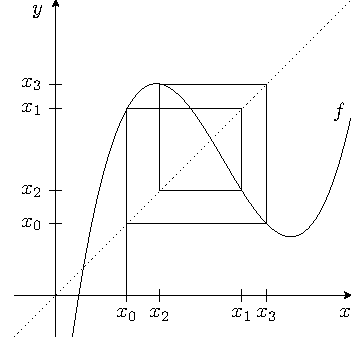
\includegraphics[]{images/iteracije_f.pdf}
% \caption[caption za v kazalo]{Dolg caption pod sliko}
  \caption[Primer vektorske slike.]{Slika prikazuje, iteracije funkcije $f$ na točki $x_0$.}
  \label{fig:iteracije}
\end{figure}

V takem dinamičnem sistemu ena iteracija funkcije predstavlja en diskreten korak v času, točka $x_0 \in I$ pa začetni položaj točke v sistemu. Množici, ki vsebuje vse člene zaporedja $\left( x_n \right)_{n=0}^{\infty}$ bomo rekli \emph{$f$-orbita točke $x_0$} ali samo orbita točke $x_0$. Z matematičnimi simboli jo lahko zapišemo tako:
$$\{ \mathcal{O} := f^m(x_0) ; m \in \N \}.$$
Izrek Šarkovskega preučuje take točke $x_0 \in I$, ki se po nekaj iteracijah s funkcijo $f$ slikajo nazaj vase. Takim točkam rečemo \emph{periodične točke}. \emph{Perioda točke} $x_0$ je najmanjše tako naravno število $m$, za katero je $f^m(x_0) = x_0$. Ekvivalentno lahko sklepamo, da je orbita periodične točke $x_0$ končna množica, število različnih elementov v orbiti pa je enako periodi točke $x_0$. Predvsem, ko želimo povdariti, da govorimo o periodični točki $x_0$, bomo $f$-orbito točke $x_0$ imenovali tudi cikel točke $x_0$. Cikel dolžine $m$ bomo krajše zapisali $m$-cikel. \emph{Negibna točka} (včasih ji rečemo tudi fiksna točka) je periodična točka s periodo 1, torej taka točka $x_0$, za katero je $f(x_0) = x_0$. Če obstaja periodična točka s periodo $n$, rečemo tudi, da ima funkcija $f$ periodo $n$.

Pri danem dinamičnem sistemu se lahko vprašamo, katere periode lahko ima funkcija. Šarkovski si je postavil prav to vprašanje in prišel do ureditve množice naravnih števil, ki pove, katere periode lahko ima funkcija.

%#############   IZREK ŠARKOVSKEGA ##############
\subsection{Izrek Šarkovskega}
Izrek šarkovskega opiše periode poljubne zvezne funkcije tako, da uredi naravna števila z relacijo delne urejenosti, ki jo moramo še spoznati.

\begin{definicija}
Naj bo $M$ množica. Relacija $(M,\leq)$ definirana na množici $M$ je relacija delne urejenosti, če veljajo naslednje lastnosti:
\begin{itemize}
\item refleksivnost: $\forall a \in M : a \leq a$,
\item antisimetričnost:  $\forall a, b \in : a \leq b \text{ in } b \leq a \Rightarrow a = b$,
\item tranzitivnost: $\forall a, b, c \in M : a \leq b \text{ in } b \leq c \Rightarrow a \leq c$.
\end{itemize}
Relacija $(M,\leq)$ je linearna urejenost, če je relacija delne urejenosti, ki je sovisna. To pomeni, da sta vsaka dva elementa v relaciji $\leq$. Natančneje: za vsak elementa $a, b \in M$ velja $a \leq b$ ali $b \leq a$.
Stroga linearna urejenost je relacija $(M, <)$, ki je tranzitivna, sovisna in irefleksivna. Irefleksivnot pomeni, da ne obstaja element $a \in M$, za katerega je $a<a$.
\end{definicija}

\begin{definicija}\label{def:ureditev-sark}
Množico naravnih števil lahko uredimo na naslednji način:
$$3 \triangleright 5 \triangleright 7 \triangleright \cdots \triangleright 2\cdot 3 \triangleright 2\cdot 5 \triangleright 2\cdot 7 \triangleright \cdots \triangleright 2^2\cdot 3 \triangleright 2^2\cdot 5 \triangleright 2^2\cdot 7 \triangleright \cdots \triangleright 2^3 \triangleright 2^2 \triangleright 2 \triangleright 1.$$
Ureditev, imenujemo jo ureditev Šarkovskega, določa relacijo $(\N, \triangleright)$, ki ji pravimo relacija Šarkovskega. Naravni števili $m$ in $n$ sta v relaciji $m\triangleright n$ (ali $n \triangleleft m$) natanko tedaj, ko $m$ leži levo od $n$ ali je $m=n$. Opazimo, da je ureditev sestavljena tako, da najprej po vrsti naštejemo liha števila večja od 1, nato dodamo ta števila po vrsti pomnožena z 2. Sledijo liha števila večja od 1 pomnožena z $2^2$ itn. Na koncu so zapisane potence števila 2 v padajočem vrstnem redu. Zaradi vrstnega reda števil pomislimo, da lahko vsako naravno število zapišemo kot produkt potence števila 2 in nekega lihega števila. To pomeni, da lahko poljubni naravni števili $m$ in $n$ zapišemo na naslednji način: 
\begin{equation}
m= 2^k(2m_1 +1)\text{ in } n= 2^l(2n_1 +1), \label{eq:zapis}
\end{equation}
 kjer so števila $m_1, n_1, k, l \in \N_0$. Števili sta v relaciji $m \triangleright n$, če je:
\begin{enumerate}[label={(R\arabic*)}]
\item $k<l$ in $m_1 \neq 0$ in $n_1 \neq 0$ ali \label{rel1}
\item $k=l$ in $0<m_1 \leq n_1$ ali \label{rel2}
\item $k \geq l$ in $m_1 = n_1=0$ ali \label{rel3}
\item $m_1>0$ in $n_1 =0$. \label{rel4}
\end{enumerate}
\end{definicija}

\begin{trditev}
Relacija $(\N, \triangleright)$, ki smo jo definirali, je relacija linearne urejenosti.
\end{trditev}
\begin{proof}
Za dokaz potrebujemo tri poljubna naravna števila:
\begin{itemize}
\item $m= 2^k(2m_1 +1)$,
\item $n= 2^l(2n_1 +1)$ in
\item $s=2^h(2s_1+1$.
\end{itemize}
Dokazati moramo refleksivnost, antisimetričnost, tranzitivnost in sovisnost relacije.
Refleksivnost: če je število $m$ liho, točka~\ref{rel3} zagotavlja, da je $m \triangleright m$. Če je število $m$ sodo, pa relacija $m \triangleright m$ sledi iz točke~\ref{rel2}.

Antisimetričnost: denimo, da za števili $m$ in $n$ veljata relaciji $m \triangleright n$ in $n \triangleright m$. Pogoja~\ref{rel1} in~\ref{rel4} za relacijo $m \triangleright n$ sta v protislovju z vsemi pogoji relacije $n \triangleright m$. Edina možnost, ki zadosti vsem potrebnim pogojem relacij je $k=l$ in $m_1 = n_1$. Torej je $m=n$.

Tranzitivnost: obravnavamo števila $m$,  $n$ in $s$, ki zadoščajo relacijam $m \triangleright n$ in $n \triangleright s$. Radi bi videli sta števili $m$ in $s$ v relaciji $m \triangleright s$. Ker imamo 4 pogoje za relacijo $m \triangleright n$ in 4 pogoje za relacijo $n \triangleright s$, moramo obravnavati 16 možnih kombinacij. Vse kombinacije pogojev za relacije so zapisane v tabeli~\ref{table:1}. V drugem stolpcu so zapisani pogoji, ki jih dobimo iz relacije $m \triangleright n$, v tretjem stoplcu so pogoji, ki jih preberemo iz relacije $n \triangleright s$. V četrti stolpec smo zapisali pogoj, ki sledi iz pogojev v drugem in tretjem stolpcu. Opazimo, da v devetih primerih pogoja ne moreta biti izpolnjena istočasno, zato pridemo do protislovja. V ostalih primerih, pa dobimo enega od pogojev za relacijo $m \triangleright s$, zato sta števili $m$ in $s$ v relaciji $m \triangleright s$.
\renewcommand{\arraystretch}{1.2}
\begin{table}[h!]
\centering
\begin{tabular}{||c | l | l | l||} 
 \hline
 Col1 & $m \triangleright n$ & $n \triangleright s$ & $\Rightarrow$ \\ [0.5ex] 
 \hline\hline
 1 & $k<l$ in $m_1, n_1 \neq 0$ & $l<h$ in $n_1, s_1 \neq 0$ & $k<h$ in $m_1, s_1 \neq 0$ \\ 
 2 & $k<l$ in $m_1, n_1 \neq 0$ & $l=h$ in $0<n_1 \leq s_1$ & $k<h$ in $m_1, s_1 \neq 0$ \\
 3 & $k<l$ in $m_1, n_1 \neq 0$ & $l \geq h$ in $n_1 = s_1 = 0$ & protislovje \\
 4 & $k<l$ in $m_1, n_1 \neq 0$ & $n_1 = 0$, $s_1 > 0$ & $m_1 = 0$, $s_1 > 0$ \\
 5 & $k=l$ in $0<m_1 \leq n_1$ & $l<h$ in $n_1, s_1 \neq 0$ & protislovje \\ 
 6 & $k=l$ in $0<m_1 \leq n_1$ & $l=h$ in $0<n_1, s_1$ & $k=h$ in $0<m_1 \leq s_1$ \\
 7 & $k=l$ in $0<m_1 \leq n_1$ & $l \geq h$ in $n_1 = s_1 = 0$ & protislovje \\
 8 & $k=l$ in $0<m_1 \leq n_1$ & $k<l$ in $n_1 = 0$, $s_1 > 0$ & $m_1 = 0$, $s_1 > 0$ \\
 9 & $k \geq l$ in $m_1 = n_1 = 0$ & $l<h$ in $n_1, s_1 \neq 0$ & protislovje \\ 
 10 & $k \geq l$ in $m_1 = n_1 = 0$ & $l=h$ in $0<n_1, s_1$ & protislovje \\
 11 & $k \geq l$ in $m_1 = n_1 = 0$ & $l \geq h$ in $n_1 = s_1 = 0$ & $k \geq h$ in $m_1 = s_1 = 0$ \\
 12 & $k \geq l$ in $m_1 = n_1 = 0$ & $k<l$ in $n_1 = 0$, $s_1 > 0$ & protislovje \\
 12 & $m_1 = 0$, $n_1 > 0$ & $l<h$ in $n_1, s_1 \neq 0$ & protislovje \\ 
 14 & $m_1 = 0$, $n_1 > 0$ & $l=h$ in $0<n_1, s_1$ & protislovje \\
 15 & $m_1 = 0$, $n_1 > 0$ & $l \geq h$ in $n_1 = s_1 = 0$ & $m_1 = 0$, $s_1 > 0$ \\
 16 & $m_1 = 0$, $n_1 > 0$ & $k<l$ in $n_1 = 0$, $s_1 > 0$ & protislovje \\[1ex] 
 \hline
\end{tabular}
\caption{Vseh 16 možnosti.}
\label{table:1}
\end{table}

Sovisnost: prepričati se moramo, da za vsaki dve naravni števili $m, n$ velja $m \triangleright n$ ali $n \triangleright m$. Torej velja en od pogojev:
\begin{enumerate}[label={(\roman*)}]
\item $k<l$ in $m_1 \neq 0$ in $n_1 \neq 0$ ali \label{sov1}
\item $k=l$ in $0<m_1 \leq n_1$ ali \label{sov2}
\item $k \geq l$ in $m_1 = n_1=0$ ali \label{sov3}
\item $m_1>0$ in $n_1 =0$ \label{sov4}
\end{enumerate}
ali 
\begin{enumerate}[label={(\roman*)}]
\setcounter{enumi}{4}
\item $l<k$ in $m_1 \neq 0$ in $n_1 \neq 0$ ali \label{sov5}
\item $l=k$ in $0<n_1 \leq m_1$ ali \label{sov6}
\item $l \geq k$ in $m_1 = n_1=0$ ali \label{sov7}
\item $n_1>0$ in $m_1 =0$. \label{sov8}
\end{enumerate}
Denimo, da števili $m$ in $n$ nista v relaciji. Iz~\ref{sov4} in~\ref{sov8} ugotovimo, da mora biti $m_1 = n_1 = 0$ ali $m_1, n_1 \neq 0$. Ker števili ne ustrezata pogoju~\ref{sov3} niti pogoju~\ref{sov7} ugotovimo, da morata biti števili $m_1$ in $n_1$ različni od 0. Iz pogojev~\ref{sov1} in~\ref{sov5} sklepamo, da mora biti $k=l$. Sedaj pa števili zagotovo zadoščata enemu od pogojev~\ref{sov2} ali~\ref{sov6}. To je preotislovje s predpostavko, da števili $m$ in $n$ nista v relaciji. Torej res za vsaki dve naravni števili $m, n$ velja relacija $m \triangleright n$ ali relacija $n \triangleright m$. 
\end{proof}

Relacija $\triangleright$ ima še eno zanimivo in za dokaz izreka Šarkovskega zelo pomembno lastnost.
\begin{trditev}\label{trd:doubling}
Števili $m$ in $n$ sta v relaciji $m \triangleright n$ natanko tedaj, ko velja relacija $2m \triangleright 2n$. Zapisano z matematičnimi simboli:
$$\text{za } \forall m, n \in \N: m \triangleright n \Leftrightarrow 2m \triangleright 2n.$$
\end{trditev}
\begin{dokaz}
Zapišimo števili $m$ in $n$ kot produkt potence števila 2 in nekega lihega števila:
$$m= 2^k(2m_1 +1)\text{ in } n= 2^l(2n_1 +1).$$
Če števili pomnožimo z 2, dobimo:
$$2m= 2^{k+1}(2m_1 +1)\text{ in } 2n= 2^{l+1}(2n_1 +1).$$
Sedaj lahko preverimo, da so pogoji za relacijo $m \triangleright n$ in relacijo $2m \triangleright 2n$ ekvivalentni. To je očitno takoj, ko opazimo, da se števili $m_1$ in $n_1$ nista spremenili. Neenačbi $k<l$ in $k+1<l+1$ pa sta ekvivalentni. Podobno ugotovimo za neenačbi $k \geq l$ in $k+1 \geq l+1$ ter enačbi $k=l$ in $k+1 = l+1$.
\end{dokaz}

Sedaj smo definirali vse potrebne pojme in spoznali tudi ureditev Šarkovskega. Čas je, da si poglejdamo, na kakšen način ureditev Šarkovskega določa periode funkcije.

\begin{izrek}[The Sharkovsky forcing theorem]\label{izr:forcing}
Če ima zvezna funkcija $f : I \to I$ točko periode $m$ in velja $ m \triangleright l$, potem obstaja tudi točka periode $l$.
\end{izrek}
Izrek pove, da je množica period zvezne funkcije na intervalu $I$ rep ureditve Šarkovskega. \emph{Rep ureditve Šarkovskega} je taka množica $\mathcal{T} \subseteq \N$, za katero je $m \triangleright n$ za  vsaki naravni števili $m \notin \mathcal{T}$ in $n \in \mathcal{T}$. Obstajajo trije različni tipi repov:  Za neko naravno število $m$ je rep množica $\{n \in \N; m \triangleright n\}$, množica $\{\dots, 16, 8, 4, 2, 1\}$ vseh potenc števila 2 in $\emptyset$.
Naslednji izrek je neke vrste obrat zgornjega izreka.

\begin{izrek}[The Sharkovsky realization theorem]\label{izr:realization}
Za vsak rep $\mathcal{T}$ v zaporedju Šarkovskega obstaja taka zvezna funkcija $f$, katere množica period je enaka $\mathcal{T}$.
\end{izrek}

Izrek Šarkovskega je unija izreka~\ref{izr:forcing} in izreka~\ref{izr:realization}. Podmnožica naravnih števil je množica period zvezne funkcije $f:I \to I$, če in samo če je množica rep ureditve Šarkovskega. Nasledja poglavja so namenjena pripravi in dokazu izreka~\ref{izr:forcing}, v poglavju~\ref{sec:realizacija} pa je predstavljen dokaz izreka~\ref{izr:realization}.

\section{Intervali, relacija pokritja in cikli}%############### Intervali, relacija pokritja in cikli
Vsi dokazi izreka Šarkovskega so si podobni po tem, da so elementarni. Ne glede na to, kako zvito se lotimo dokaza, je ključnega pomena lastnost zveznih funkcij, ki ob določenih predpostavkah zagotavlja obstoj ničle funkcije. To je izrek o vmesni vrednosti.

\begin{izrek}[izrek o vmesni vrednosti]\label{izr:iovv}
Funkcija $f$, ki je zvezna na intervalu $[a, b]$ in je na krajiščih intervala različno predznačena, torej velja neenačba $f(a)\cdot f(b) < 0$, ima vsaj v eni točki tega intervala vrednost 0.
\end{izrek}

\begin{figure}[h]
  \centering
  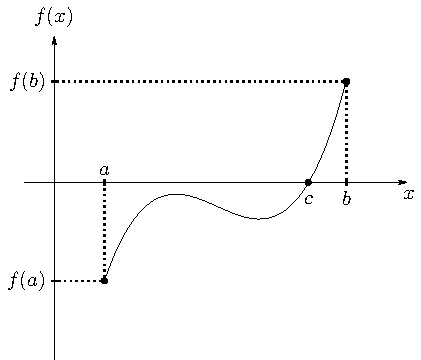
\includegraphics[]{images/intermediate.pdf}
% \caption[caption za v kazalo]{Dolg caption pod sliko}
  \caption[Primer vektorske slike.]{Slika prikazuje, kako poiščemo interval $K$.}
  \label{fig:bezje}
\end{figure}

\begin{proof}
Naj bo funkcija $f:[a, b] \to [a, b]$ zvezna in naj bo $f(a)\cdot f(b) < 0$. Brez izgube splošnosti lahko predpostavimo, da je $f(a) < 0 < f(b)$. Ničlo funkcije $f$ bomo iskali s pomočjo deljenja intervalov oziroma z bisekcijo. Izračunamo razpolovišče $p_0=\frac{a+b}{2}$ intervala $[a, b]$.Če je $f(p_0)=0$, smo ničlo že našli, sicer razmišljamo tako: če je $f(p_0) >0$, označimo $[a_1, b_1] =  [a, p_0]$, sicer označimo $[a_1, b_1] =  [p_0, b]$. Nato izračunamo razpolovišče $p_1$ intervala $[a_1, b_1]$. Če je $f(p_1)=0$ postopek ustavimo, saj smo ničlo našlio, v nasprotnem primeru pogledamo predznak $f(p_1)$. Če je $f(p_1) >0$, označimo $[a_2, b_2] =  [a_1, p_1]$, drugače označimo $[a_2, b_2] =  [p_1, b_1]$. Postopek nadaljujemo dokler ne najdemo ničle $p_i$ funkcije $f$. Če ničle ne najdemo, dobimo neskončno zaporedje vloženih intervalov 
$$ [a, b] \supset [a_1, b_1] \supset [a_2, b_2] \supset \cdots$$
Lahko se prepričamo, da je $b_n - a_n = \frac{b-a}{2^n}$ in $f(a_n)<0<f(b_n)$ za vsak $n\in \N$. Števila $a_n$ tvorijo naraščajoče zaporedje, števila $b_n$ pa padajoče zaporedje.  Limiti $\lim\limits_{n \to \infty} a_n$ in $\lim\limits_{n \to \infty} b_n$ sta enaki, saj je 
$\lim\limits_{n \to \infty} b_n - \lim\limits_{n \to \infty} a_n = \lim\limits_{n \to \infty} (b_n - a_n) = \lim\limits_{n \to \infty} \frac{b - a}{2^n} = 0$. Označimo $c = \lim\limits_{n \to \infty} a_n = \lim\limits_{n \to \infty} b_n$. Točka $c$ je večja od vseh členov zaporedja $\left(a_n \right)_{n=1}^{\infty}$ in manjša od vseh členov zaporedja $\left(b_n \right)_{n=1}^{\infty}$, zato je za vsak $n \in \N$ vsebovana v intervalu $[a_n, b_n]$. Torej velja:
$\bigcap\limits_{n=1}^{\infty} [a_n, b_n] = \{c\}$. 
Ker je funkcija zvezna, je 
$\lim\limits_{n \to \infty} f(a_n) = f\left(\lim\limits_{n \to \infty} a_n\right) = f(c)$
in 
$\lim\limits_{n \to \infty} f(b_n) = f\left(\lim\limits_{n \to \infty} b_n\right) = f(c)$.
Za vsako naravno število $n$ velja $f(a_n) <0$, zato je $f(c) \leq 0$. Podobn je $f(b_n) > 0$ za vsako naravno število $n$, iz česar sklepamo, da je $f(c) \geq 0$. Torej je $f(c) = 0$, kar zaključi dokaz.
\end{proof}

\begin{posledica}\label{pos:vmesnavrednost}
Naj bo $f : [a, b] \to [a, b]$ zvezna funkcija. Za vsako točko $y$, ki leži med točkama $f(a)$ in $f(b)$, obstaja točka $c \in (a, b)$, za katero je vrednost funkcije $f(c)$ enaka $y$.
\end{posledica}
\begin{proof}
Definiramo zvezno funkcijo $g(x) = f(x) - y$. Ker točka $y$ leži med točkama $f(a)$ in $f(b)$, je funkcija $g$ na krajiščih intervala $[a, b]$ različno predznačena. Po izreku~\ref{izr:iovv} obstaja točka $c$, za katero je $g(c) = 0$. To pomeni, da je $f(c) = y$.
\end{proof}
Posledica pove, da zvezna funkcija na intervalu $[a, b]$ zavzame vse vrednosti med $f(a)$ in $f(b)$. V resnici pove še več. Naj bosta $[a, b]$ in $[c, d]$ intervala v realnih številih in $f : [a, b] \to \R$ zvezna funkcija. Če obstajata taki točki $a_1, b_1 \in [a, b]$, za kateri velja $f(a_1) \leq c$ in $f(b_1) \geq d$, potem interval $[c, d]$ leži v sliki $f([a, b])$. To je res, saj funkcija $f$ na intervalu $[a_1, b_1]$ zavzame vse vrednosti med $f(a_1)$ in $f(b_1)$. Torej, $[c, d] \subset f([a_1, b_1]) \subset f([a, b])$.

\begin{definicija}\label{def:pokritja}
Pravimo, da interval $I$ pokrije interval $J$, če je $J \subseteq f(I)$. Relacijo zapišemo kot $I \xrightarrow{f} J$. Kadar je jasno, katera funkcija nastopa v relaciji, lahko nadpis, ki označi katero funkcijo imamo v mislih tudi izpustimo in pišemo samo $I \to J$. Če velja $f(I) =J$, zapišemo $I \rightarrowtail J$.
\end{definicija}
S pomočjo izreka o vmesni vrednosti in poznavanja, kako se intervali slikajo s funkcijo $f$, lahko izvemo, ali obstajajo periodične točke. Kako potrdimo obstoj periodičnih točk, nam povejo naslednje leme.

\begin{lema}\label{lem:1zanka}
Če velja $[a, b] \xrightarrow{f} [a, b]$, potem ima funkcija $f$ negibno točko na intervalu $[a, b]$.
\end{lema}
\begin{proof}
Interval $[a, b]$ je podmnožica slike $f([a, b])$, zato obstajata taki točki $a_1, b_1 \in [a, b]$, da je $f(a_1)=a$ in $f(b_1)=b$. Če je $a_1 = a$ ali $b_1 = b$, smo negibno točko že našli. Če je $a_1 \neq a$ in $b_1 \neq b$, definiramo funkcijo $g(x) = f(x) - x$. Prepričajmo se, da je vrednost funkcije $g$ v točki $a_1$ negativna, v točki $b_1$ pa pozitivna. Računamo:
$g(a_1) = f(a_1) - a_1 = a - a_1 < 0$. Podobno je
$g(b_1) = f(b_1) - b_1 = b - b_1 > 0$.
Zvezna funkcija $g$ je na krajiščih intervala $[a, b]$ različno predznačena. Po izreku~\ref{izr:iovv} obstaja točka $c \in [a, b]$, pri kateri je $g(c)=0$, torej je $f(c) = c$.
\end{proof}
Pri iteracijah funkcije lahko opazujemo, kako se premika točka. To smo počeli na sliki~\ref{fig:iteracije}. Poglejmo, kako se s $f$ slikajo celi intervali. Lahko se zgodi, da nek interval $I_0$ pokrije interval $I_1$, interval $I_1$ pa pokrije interval $I_2$ itn. Na ta način dobimo zaporedje relacij pokritja npr. $I_0 \to I_1 \to I_2 \to \cdots $ Enako kot pri periodičnih točkah lahko pri zaporedju relacij pokritja po nekaj korakih zopet pridemo do prvotnega intervala. Dobimo naslednje zaporedje relacij pokritja: $I_0 \to I_1 \to \cdots \to I_n \to I_0$. Če je začetni interval enak končnemu intervalu, zaporedju intervalov in pripadajočim relacijam pokritja pravimo \emph{zanka intervalov} ali samo zanka. Od tu naprej bo, razen če ne povemo drugače, interval predstavljal zaprto, omejeno in povezano podmnožico realnih števil.

\begin{lema}\label{lem:zanka}
Če za intervale $I_0, I_1, \dots, I_{n-1}$ veljajo naslednje relacije pokritosti: $I_0 \to I_1 \to \dots \to I_{n-1} \to I_0$, potem obstaja taka točka $c \in I_0$, za katero je $f^{i}(x) \in I_i$ za $0 \leq i < n$ in $f^n(c)=c$. Pravimo, da točka $c$ sledi zanki.
\end{lema}

\begin{proof}
Če velja relacija pokritosti $I \to J$, obstaja tak interval $K \subset I$, da je $K \rightarrowtail J$.
\begin{figure}[h]
  \centering
  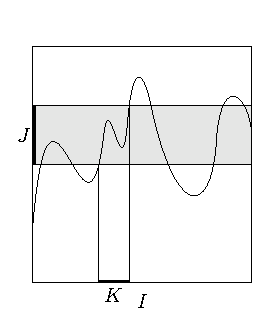
\includegraphics[]{images/bezje.pdf}
% \caption[caption za v kazalo]{Dolg caption pod sliko}
  \caption[Primer vektorske slike.]{Slika prikazuje, kako poiščemo interval $K$.}
  \label{fig:bezje}
\end{figure}
Interval $K$ poiščemo tako, da iz preseka funkcije $f$ s pravokotnikom $I \times J$ izberemo povezan del grafa, ki povezuje spodni in zgornji del pravokotnika. Tak del zagotovo obstaja, saj je $J \subset f(I)$. Projekcijo tega dela na interval $I$ označimo s $K$. To znanje uporabimo na zanki intervalov $I_0 \to \dots \to I_{n-1} \to I_0$. Ker velja relacija pokritja $I_{n-1} \to I_0$, vemo, da obstaja tak interval $K_{n-1} \subset I_{n-1}$, da je $K_{n-1} \rightarrowtail I_0$. Velja relacija pokritosti $I_{n-2} \to K_{n-1}$, zato obstaja tak interval $K_{n-2} \subset I_{n-2}$, da je $K_{n-2} \rightarrowtail K_{n-1}$. S postopkom nadaljujemo in dobimo naslednje relacije:
$$K_0 \rightarrowtail K_1 \rightarrowtail \cdots \rightarrowtail K_{n-1} \rightarrowtail I_0.$$
Za vsako točko $x \in K_0$ in za vsak $i \in [0, n)$ velja $f^i(x) \in K_i \subset I_i$ in $f^n(x) \in I_0$. Ker je $K_0 \subset I_0 = f^n(K_0)$, lahko s pomočjo leme~\ref{lem:1zanka} sklepamo, da ima $f^n$ negibno točko $c$ na intervalu $K_0$. Točka $c$ sledi zanki $I_0 \to I_1 \to \dots \to I_{n-1} \to I_0$.
\end{proof}

Pri dokazovanju izreka bomo dokazali obstoj zank različnih dolžin. Želeli bi si, da je perioda točke, ki sledi zanki, enaka dolžini zanke. 

\begin{definicija}\label{def:element}
Zanka intervalov $I_0 \to I_1 \to \cdots \to I_{n-1} \to I_0$ je elementarna, če ima vsaka točka, ki sledi zanki, periodo $n$.
\end{definicija}

\begin{posledica}
Vsaka elementarna zanka intervalov $I_0 \to I_1 \to \dots \to I_{n-1} \to I_0$ vsebuje točko $x_0$, ki sledi zanki in ima periodo $n$.
\end{posledica}

Zaradi zgornje posledice bi bilo dobro, če bi poznali kakšen kriterij za prepoznavanje elementarnih zank. Najlažji kriterij je število intervalov v zanki. Če nastopa samo en interval, dobimo zanko $I_0 \to I_0$. Z uporabo leme~\ref{lem:1zanka} ugotovimo, da je zanka elementarna. Naslednja lema poda še en kriterij za prepoznavanje elementarnih zank:

\begin{lema}\label{lem:element}
Zanka intervalov $I_0 \to I_1 \to \cdots \to I_{n-1} \to I_0$ je elementarna, če ji ne sledi nobena robna točka intervala $I_0$ in je notranjost intervala $\interior(I_0)$ disjunktna z intervali $I_1, I_2,  \dots, I_{n-1}$. Torej, $\interior(I_0) \cap \bigcup_{i=1}^{n-1}I_i = \emptyset$.
\end{lema}
\begin{proof}
Točka $x_0$, ki sledi zanki, ne more biti robna točka intervala $I_0$. Torej je $x_0 \in \interior(I_0)$. Za vsak $i=1, \dots, n-1$ je $x_0 \neq f^i(x_0)$, saj je $f^i(x_0) \in I_i$, notranjost intervala $I_0$ pa je disjunktna z intervalom $I_i$. Ker točka $x_0$ sledi zanki, je $f^n(x_0)=x_0$. Točka $x_0$ ima periodo $n$.
\end{proof}

Poglejmo si dva primera, ki pokažeta, da nobene predpostavke v lemi~\ref{lem:element} ne moremo izpustiti.

\begin{primer}\label{prim:robna}
Obravnavajmo zvezno funkcijo $f(x) = -\sqrt[3]{x}$ in 2-zanko intervalov $\left[0, \frac{1}{2}\right] \leftrightarrows \left[-\frac{1}{2}, 0\right]$. Samo ena točka sledi tej zanki, to je točka 0. Perioda točke 0 ni enaka enaka dolžini zanke, saj je točka 0 negibna točka in je njena perioda enaka 1.
\end{primer}
\begin{primer}\label{prim:notranja}
Funkcija $f(x) = - x^2$ tvori $2$-zanko $\left[\frac{1}{4}, \frac{9}{4}\right] \leftrightarrows \left[\frac{1}{2}, 4\right]$. Tej zanki sledi zgolj točka $1$, ki je negibna točka, torej je njena perioda različna od dolžine zanke.
\end{primer}
Zanka v primeru~\ref{prim:robna} ni elementarna, saj ji sledi robna točka začetnega intervala. V primeru~\ref{prim:notranja} pa zanka ni elementarna, saj točka 1 leži v preseku notranjosti prvega intervala in drugega intervala. 

\begin{definicija}
Zaprt in omejen interval, katerega krajišči pripadata ciklu $\mathcal{O}$ imenujemo $\mathcal{O}$-interval. 
\end{definicija}
V nadaljevanju bomo zgornje leme uporabili na $\mathcal{O}$-intervalih. Tako bomo poenostavili obravnavo periodičnih točk funkcije $f$, saj bomo uporabili samo informacije, ki jih lahko pridobimo iz delovanja funkcije $f$ na ciklu $\mathcal{O}$. Zato bodo naši sklepi veljali za vse zvezne funkcije s ciklom $\mathcal{O}$. Relaciji pokritja $I \to J$ rečemo $\mathcal{O}$-vsiljena, če interval $J$ leži v $\mathcal{O}$-intervalu $M$, katerega krajišči sta skrajno leva in skrajno desna točka množice $f(I \cap \mathcal{O})$. Ker je funkcija $f$ zvezna, lahko s pomočjo izreka~\ref{izr:iovv} ugotovimo, da je množica $f(I)$ interval. Velja $J \subset M \subset f(I)$. V nadaljevanju dela bodo vse relacije pokritja $\mathcal{O}$-vsiljene. Zanka intervalov $I_0 \to I_1 \to \cdots \to I_{n-1} \to I_0$, v kateri vsaka puščica predstavlja $\mathcal{O}$-vsiljeno relacijo pokritja, se imenuje $\mathcal{O}$-vsiljena zanka $\mathcal{O}$-intervalov.

%Vse relacije pokritja, o katerih bomo govorili, bodo $\mathcal{O}$-vsiljene, zato bodo vse relacije pokritja, ki jih bomo označili s simbolom `$\to$', predstavljale $\mathcal{O}$-vsiljene relacije pokritja.

Vse relacije pokritja, o katerih bomo govorili od sedaj naprej in jih bomo označevali s simbolom `$\to$' bodo $\mathcal{O}$-vsiljene.

%################ POGLAVJE S PRIMERI ##############
\section{Primeri}
V tem poglavju si bomo zaradi lažjega razumevanja pogledali nekaj posebnih primerov. Najprej si bomo pogledali najbolj znan poseben primer izreka Šarkovskega. V naslednjih dveh primerih bomo postopek iz prvega primera razširili na daljše cikle. V zadnjem primeru bomo nakazali, kako lahko iz periodičnih točk funkcije $f^2$ ugotovimo, katere periode ima funkcija $f$, kar igra pomembno vlogo pri dokazu izreka~\ref{izr:forcing}.

\begin{primer}[3-cikel]\label{primer1}
Prepričajmo se, da perioda 3 implicira obstoj vseh ostalih period. Točka lahko tvori $3$-cikel na dva različna načina, ki sta v resnici zrcalna podoba drug drugega. Slika~\ref{fig:3cikla} prikazuje oba primera. 
\begin{figure}[h]
  \centering
  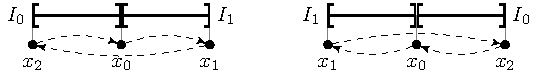
\includegraphics{images/tricikel.pdf}
% \caption[caption za v kazalo]{Dolg caption pod sliko}
  \caption[Primer vektorske slike.]{Zrcalna podoba ciklov.}
  \label{fig:3cikla}
\end{figure}
Črtkane puščice nakazujejo, kam se s funkcijo $f$ slikajo točke. Velja: 
$$x_1 = f(x_0), x_2 = f(x_1) \text{ in } x_0 = f(x_2).$$
V obeh primerih smo z $I_1$ označili $\mathcal{O}$-interval s krajišči $x_0$ in $x_1$, z $I_0$ pa $\mathcal{O}$-interval s krajišči $x_0$ in $x_2$. Krajišči intervala $I_1$ se slikata v skrajno levo in skrajno desno točko cikla, zato imamo $\mathcal{O}$-vsiljeni pokritji $I_1 \to I_1$ in $I_1 \to I_0$. Krajišči intervala $I_0$ se slikata v krajišči intervala $I_1$, zato je tudi pokritje $I_0 \to I_1$ $\mathcal{O}$-vsiljeno. Ugotovljena pokritja lahko strnemo v diagram $\sara I_1 \leftrightarrows I_0$. Iz relacije pokritosti $I_1 \to I_1$ in leme~\ref{lem:1zanka} sklepamo, da interval $I_1$ vsebuje negibno točko. Krajišči intervala $I_0$ ne morejo slediti zanki $I_0 \to I_1 \to I_0$, saj sta periodični točki s periodo 3. Točke, ki sledijo zanki, pa imajo periodo 1 ali 2. Ker je notranjost intervala $I_0$ disjunktna z intervalom $I_1$, lahko s pomočjo leme~\ref{lem:element} sklepamo, da je zanka elementarna. Torej lahko v intervalu $I_0$ poiščemo točko s periodo 2. Za dokaz obstoja točke s periodo $l\geq 4$ si poglejmo zanko
\begin{equation}
I_0 \to \overbrace{I_1 \to I_1 \to \cdots \to I_1}^{l-1 \text{ ponovitev intervala } I_0} \to I_0. \label{eq:lzanka}
\end{equation}
V tej zanki nastopajo vsaj 3 kopije intervala $I_1$, v katerem ležita samo dve točki $\mathcal{O}$-intervala. Ker imajo točke iz cikla $\mathcal{O}$ periodo 3, v intervalu $I_1$ ne morejo ležati trije zaporedni členi iz cikla $\mathcal{O}$, torej tudi tri zaporedne iteracije funkcije $f$ na krajiščih intervala $I_0$ ne morejo ležati v intervalu $I_1$. To pomeni, da krajišči intervala $I_0$ ne moreta slediti zanki. Že prej smo ugotovili, da je notranjost intervala $I_0$ disjunktna z intervalom $I_1$, zato je zanka~\eqref{eq:lzanka} elementarna zanka dolžine $l$. Elementarna $l$-zanka vsebuje točko periode $l$, torej ima funkcija $f$ periodo $l$ za vsak $l \geq 4$. Pokazali smo, da je vsako naravno število perioda funkcije $f$.
\end{primer}


\begin{primer}[7-cikel] \label{primer2}
Sedaj bomo obravnavali 7-cikel $\mathcal{O}$ in $\mathcal{O}$-intervale prikazane na sliki~\ref{fig:7cikel}.
\begin{figure}[h]
  \centering
  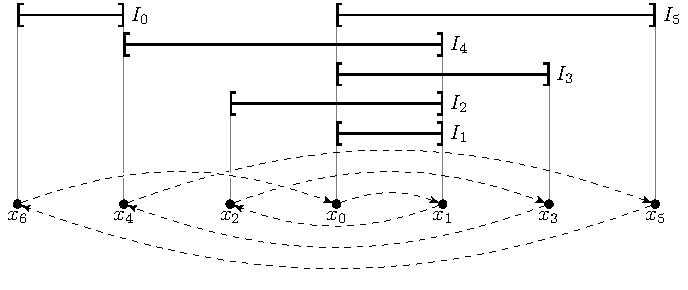
\includegraphics{images/sedemcikel.pdf}
% \caption[caption za v kazalo]{Dolg caption pod sliko}
  \caption[Primer vektorske slike.]{Primer 7-cikla.}
  \label{fig:7cikel}
\end{figure}
 Podobno kot pri prejšnjem primeru označimo točke $x_i = f^i(x_0)$ ter intervale $I_1 = [x_0, x_1]$, $I_2 = [x_1, x_2]$  in tako naprej kot prikazuje slika~\ref{fig:7cikel}. Za to izbiro intervalov dobimo naslednje $\mathcal{O}$-vsiljene relacije pokritosti:
\begin{enumerate}
\item $I_1 \to I_1$
\item $I_1 \to I_2 \to I_3 \to I_4 \to I_5 \to I_0$
\item $I_0 \to I_1$, $I_0 \to I_3$ in $I_0 \to I_5$
\end{enumerate}
Zgornje relacije pokritosti lahko prikažemo z grafom, ki ga prikazuje slika~\ref{fig:6kotnik}.
\begin{figure}[h]
  \centering
  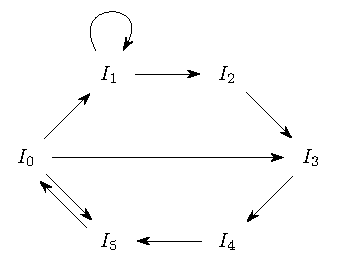
\includegraphics{images/graph6.pdf}
% \caption[caption za v kazalo]{Dolg caption pod sliko}
  \caption[Primer vektorske slike.]{diagram}
  \label{fig:6kotnik}
\end{figure}
Iz grafa preberemo naslednje zanke.
\begin{enumerate}[label={(\arabic*)}]
\item $I_1 \to I_1$
\item $I_0 \to I_5 \to I_1$ \label{7cikelz2}
\item $I_0 \to I_3 \to I_4 \to I_5 \to I_0$ \label{7cikelz3}
\item $I_0 \to I_1 \to I_2 \to I_3 \to I_4 \to I_5 \to I_0$ \label{7cikelz4}
\item $I_0 \to \underbrace{I_1 \to I_1 \to \cdots  \to I_1}_{r \text{ ponovitev intervala } I_1} \to I_2 \to I_3 \to I_4 \to I_5 \to I_0$, kjer je $r\geq 3$. \label{7cikelz5}
\end{enumerate}
Zanka $I_1 \to I_1$ je elementarna, saj je elementarna vsaka zanka dolžine 1. Pri ostalih zankah lahko najprej ugotovimo, da za vsak $j \in \{1, 2, \dots, 5\}$ velja $\interior(I_0) \cap I_j = \emptyset$. Pri zankah~\ref{7cikelz2},~\ref{7cikelz3} in~\ref{7cikelz4} nobena robna točka intervala $I_0$ ne more slediti zanki, saj je perioda robnih točk 7, perioda točk, ki sledijo zankam~\ref{7cikelz2},~\ref{7cikelz3} in~\ref{7cikelz4} pa je manjša ali enaka 6. S tem so izpolnjeni pogoji leme~\ref{lem:element} in so zanke elementarne. V teh zankah lahko poiščemo točke s periodami 2, 4, ali 6. Podobno kot v primeru~\ref{primer1} ugotovimo, da nobene tri zaporedne iteracije funkcije $f$ na točkah cikla $\mathcal{O}$ ne ležijo v intervalu $I_1$, zato v tem intervalu tudi ne morejo ležati tri zaporedne iteracije funkcije $f$ na robnih točkah intervala $I_0$. To pomeni, da krajišči intervala $I_0$ ne sledita zanki~\ref{7cikelz5}. S tem razmislekom so izpolnjeni pogoji leme~\ref{lem:element}, zato je zanka~\ref{7cikelz5} elementarna. Za dolžino zanke~\ref{7cikelz5} lahko izberemo katerokoli naravno število večje od 7. Torej lahko na podlagi prisotnosti 7-cikla na sliki~\ref{fig:7cikel} sklepamo, da so prisotne vse periode $l$, za katere je $l \triangleleft 7$
\end{primer}

\begin{primer}[9-cikel] \label{primer3}
Predpostavimo, da ima funkcija $f$ 9-cikel $\mathcal{O}$, ki je prikazan na sliki~\ref{fig:9cikel}. 
\begin{figure}[h]
  \centering
  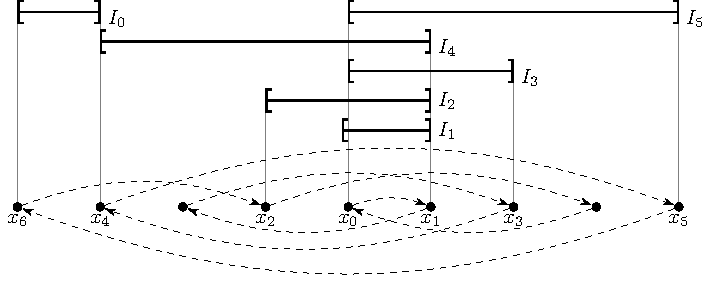
\includegraphics{images/devetcikel.pdf}
% \caption[caption za v kazalo]{Dolg caption pod sliko}
  \caption[Primer vektorske slike.]{Primer 9-cikla.}
  \label{fig:9cikel}
\end{figure}
Določili smo šest $\mathcal{O}$-intervalov $I_0, I_1, \dots, I_5$, za katere velja, da je notranjost intervala $I_0$ disjunktna z ostalimi intervali. Torej za $j=1, 2, \dots, 5$ velja enakost: $\interior{(I_0)} \cap I_j = \emptyset$. Za tako izbrane intervale dobimo enake relacije pokritja kot v primeru~\ref{primer1} in lahko s pomočjo enakih sklepov ugotovimo prisotnost enakih elementarnih zank in posledično periodičnih točk s periodami 1, 2, 4, 6 in vse periode večje od 7.

Zaporedje števil $x_0, x_1, \dots, x_6$ smo določili tako, da se spiralno oddaljujejo od centra $c:=\frac{x_0+x_1}{2}$, kar je prikazano na sliki~\ref{fig:spiral}. S tako izbiro točk pa v zaporedju ne nastopajo vse točke cikla $\mathcal{O}$ in tudi ne velja enakost $f(x_i) = x_{i+1}$ za vsak $i = 1, 2, \dots, 5$ kot je to veljalo v primeru~\ref{primer2}.

\begin{figure}[h]
  \centering
  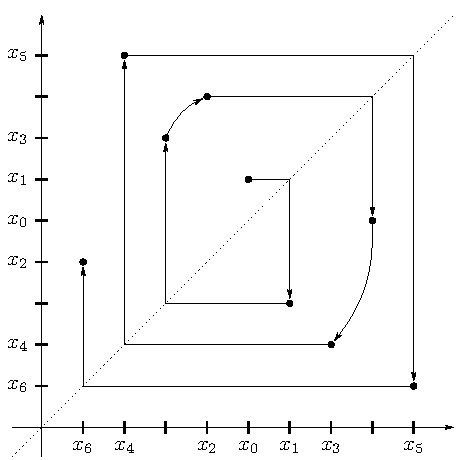
\includegraphics{images/spiral.pdf}
% \caption[caption za v kazalo]{Dolg caption pod sliko}
  \caption[Primer vektorske slike.]{Primer 9-cikla.}
  \label{fig:spiral}
\end{figure}

V poglavju~\ref{konssz} je predstavljen algoritem za izbiro zaporedja točk $x_0, x_1, \dots, x_6$. Glavna ideja algoritma je, da za naslednji člen zaporedja ne izberemo vedno sliko prejšnjega člena na način: $x_{i+1} = f(x_i)$, vendar včasih izberemo točko, ki je bližje centru $c$. Točko $x_{i+1}$, ki je bližje centra $c$ kot točka $f(x_i)$ izberemo, če je slika $f(x_{i+1})$ bolj oddaljena od centra kot točka $f(f(x_i))$. Postopka izbire naslednje točke na sliki~\ref{fig:iteracije} in na sliki~\ref{fig:spiral} sta podobna. V obeh primerih se pomikamo navpično do grafa funkcije in nato vodoravno do simetrale lihih kvadrantov. Sprememba se zgodi na sliki~\ref{fig:spiral}, ko lahko izberemo še neizbrano točko tako, da se v vodoravni smeri pomaknemo proti centru $c$, v navpični smeri pa stran od centra $c$. To se na sliki~\ref{fig:spiral} zgodi dvakrat in je prikazano s krivimi puščicami. 
Postopek se ustavi, ko pridemo do točke $x_j$, katere slika $f(x_j)$ je na isti strani centra $c$ kot točka sama. V primeru na sliki~\ref{fig:spiral} je to točka $x_6$.

V poglavju~\ref{stefan_zap} si bomo natančno pogledali kakšne lastnosti mora imeti zaporedje točk $x_0, x_1, \dots, x_{n-1}$, ki predstavlja krajišča intervalov $I_0, I_1, \dots, I_{n-1}$. Izvedeli bomo tudi, kako taka izbira točk in intervalov zagotavlja obstoj elementarnih zank. V poglavju~\ref{konsz} se bomo naučili, kako iz točk cikla izberemo zaporedje, ki ima željene lastnosti. 

\end{primer}

\begin{primer}[6-cikel] \label{primer4}
Obravnavali bomo 6-cikel, ki je na sliki~\ref{fig:6cikel}. 
 \begin{figure}[h]
  \centering
  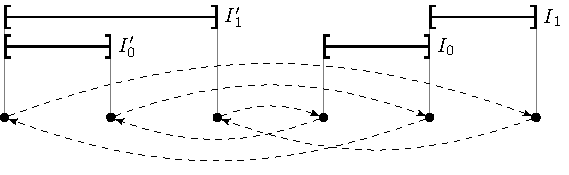
\includegraphics{images/sestcikel.pdf}
% \caption[caption za v kazalo]{Dolg caption pod sliko}
  \caption[Primer vektorske slike.]{Primer 6-cikla.}
  \label{fig:6cikel}
\end{figure}
Bistveno pri tem primeru je, da se tri točke na levi strani slikajo v tri točke na desni in obratno. Torej, tri točke na desni tvorijo 3-cikel
\tikz{
\tikzset{vertex/.style = {shape=circle, fill=black,draw,minimum size=3pt, inner sep=0pt}}
\tikzset{edge/.style = {->,> = latex'}}
	\node [vertex](1) at  (0, 0) {};
	\node[vertex] (2) at  (0.8, 0) {};
	\node[vertex] (3) at  (1.6, 0) {};
	\draw[edge, dashed] (1) to[bend left=20] (2);
	\draw[edge, dashed] (2) to[bend left=20] (3);
	\draw[edge, dashed] (3) to[bend left=15] (1);
}
 za funkcijo $f^2$. Podobno kot v primeru~\ref{primer1} lahko določimo intervala $I_0$ in $I_1$ ter opazujemo relacije pokritja $I_1 \xrightarrow{f^2} I_1$, $I_1 \xrightarrow{f^2} I_0$ in $I_0 \xrightarrow{f^2} I_1$ za intervala $I_0$ in $I_1$, ki sta prikazana na sliki~\ref{fig:6cikel}. Enako kot prej lahko zaključimo, da ima funkcija $f^2$ elementarne zanke vseh dolžin in zato je vsako naravno število $l \in \N$ perioda funkcije $f^2$. Za funkcijo $f$ določimo še dva intervala. Interval $I_0'$ naj bo najkrajši $\mathcal{O}$-interval, ki vsebuje točke iz množice $f(I_0 \cup \mathcal{O})$, interval $I_1'$ pa naj bo najkrajši $\mathcal{O}$-interval, ki vsebuje točke iz množice $f(I_1 \cup \mathcal{O})$. Sedaj bomo prikazali rekurzivno metodo, ki jo bomo uporabili kasneje v dokazu izreka Šarkovskega. Pokazali bomo, kako lahko s pomočjo elementarne $k$-zanke za funkcijo $f^2$ poiščemo elementarno $2k$-zanko za funkcijo $f$. V primeru, ki ga obravnavamo, bo to pomenilo, da je vsako sodo naravno število perioda funkcije $f$.
Poglejmo si elementarno $k$-zanko za funkcijo $f^2$, v kateri nastopajo relacije pokritja 
$I_1 \xrightarrow{f^2} I_1$, $I_1 \xrightarrow{f^2} I_0$ in $I_0 \xrightarrow{f^2} I_1$. Vsak zapis $I_1 \xrightarrow{f^2}$ v zanki lahko zamenjamo z $I_1 \xrightarrow{f} I_1'  \xrightarrow{f}$, vsak zapis $I_0 \xrightarrow{f^2} $ pa z $I_0 \xrightarrow{f} I_0'  \xrightarrow{f}$. S to spremembo dobimo $2k$-zanko za funkcijo $f$, ki ni samo dvakrat ponovljena $k$-zanka. Prepričajmo se, da je $2k$-zanka elementarna. Denimo, da točka $p$ sledi $2k$-zanki za funkcijo $f$. Pokazati moramo, da ima periodo $2k$ za funkcijo $f$. Opazimo, da točka $p$ sledi prvotni $k$-zanki za funkcijo $f^2$ in ima zato periodo $k$ za funkcijo $f^2$. Po drugi strani pa iteracije točke $p$ s funkcijo $f$ ležijo alternirajoče enkrat na levi in enkrat na desni strani srednjega intervala, saj $2k$-zanka za $f$ alternira med intervali s črtico in intervali brez črtice. Zato je orbita točke $p$ sestavljena iz $2k$ različnih točk. Na desni strani srednjega intervala leži $k$ sodih iteracij, na levi strani pa leži $k$ lihih iteracij. To pomeni, da je perioda točke $p$ za $f$ enaka $2k$. Ker smo dolžino začetne elementarne $k$-zanke izbrali poljubno, smo pokazali, da je vsako sodo število perioda za $f$. Ker interval $[x_0, x_1]$ s funkcijo $f$ pokrije samega sebe, pa obstaja negibna točka. Torej ima $f$ tudi periodo 1. 
\end{primer}

%################################## ŠTEFANOVO ZAPOREDJE ###########################
%##############################################################################
\section{Štefanovo zaporedje} \label{stefan_zap} 
V tem poglavju bomo podali definicijo Štefanovega zaporedja točk. Pokazali bomo, da te točke določajo intervale, s pomočjo katerih lahko zapišemo relacije pokritja in ustrezne zanke, ki zagotavljajo obstoj periodičnih točk. 
Če $f$-orbita vsebuje samo eno točko, je ta točka fiksna točka funkcije $f$. Perioda te točke je 1, kar je zadnji člen ureditve Šarkovskega in pri tej orbiti nimamo kaj dokazovati. Zato bomo obravnavali samo orbite oziroma cikle, ki vsebujejo vsaj dve točki. Naj bo $m \geq 2$ in $\mathcal{O}$ $m$-cikel zvezne funkcije $f$. Preden definiramo Štefanovo zaporedje, moramo spoznati nekaj pojmov. 

\begin{definicija}
Naj bo $p$ najbolj desna točka $m$-cikla $\mathcal{O}$, za katero je $f(p) > p$ in $q\in \mathcal{O}$ prva točka desno od p. Center $c$ cikla $\mathcal{O}$ definiramo kot $c=\frac{p+q}{2}$. Za vsako točko $x \in \mathcal{O}$ označimo množico točk iz cikla $\mathcal{O}$, ki ležijo v zaprtem intervalu omejenem z $x$ in $c$, z $\mathcal{O}_x$. Natančneje, $\mathcal{O}_x = \mathcal{O} \cap [x, p]$, če je $x \leq p$ in  $\mathcal{O}_x = \mathcal{O} \cap [q, x]$, če je $x \geq q$. Pravimo, da točka $x \in \mathcal{O}$ menja strani, če točka $c$ leži med točkama $x$ in $f(x)$.
\end{definicija}
Poglejmo si definicijo Štefanovega zaporedja.

\begin{definicija}\label{def:stef}
Iz $m$-cikla $\mathcal{O}$ izbrane točke $x_0, x_1, \dots, x_n$ tvorijo Štefanovo zaporedje, če je:

\begin{enumerate}[label={(Š\arabic*)}]
    \item $\{x_0, x_1\} = \{p, q\}$, \label{eq:š1}
    \item točke $x_0, x_1, \dots, x_n$ ležijo alternirajoče na levi oziroma desni strani točke $c$, \label{eq:š2}
    \item zaporedji 
    $\left \{ x_{2j} \right \}_{j=0}^{\left \lfloor \frac{n}{2} \right \rfloor}$ 
    in
    $\left \{ x_{2j+1} \right \}_{j=0}^{\left \lfloor \frac{n}{2} \right \rfloor}$ sta strogo monotoni in se oddaljujeta od točke $c$, \label{eq:š3}
    \item če je $0\leq j \leq n-1$, potem $x_j$ menja strani in $x_{j+1} \in \mathcal{O}_{f(x_j)}$,\label{eq:š4}
    \item točka $x_n$ ne menja strani. \label{eq:š5}
\end{enumerate}
  
\end{definicija}
\begin{opomba}\label{op:štefzap}
Štefanovo zaporedje dobimo tako, da iz množice $m$ točk, ki tvorijo $\mathcal{O}$-cikel izberemo $n+1$ točk, ki zadoščajo zgornjim pogojem. 
Pogoj $x_{j+1} \in \mathcal{O}_{f(x_j)}$ v~\ref{eq:š4} pomeni, da je točka $x_{j+1}$ bližje centru kot slika $f(x_j)$ točke $x_j$. Velja ena od neenakosti: $c < x_{j+1} \leq f(x_j)$ ali $f(x_j) \leq x_{j+1} < c$. Pogoja ~\ref{eq:š2} in~\ref{eq:š3} zagotavljata, da so točke $x_0, x_1, \dots, x_n$ paroma različne. Če sledimo točkam na način, ki je opisan v primeru~\ref{primer3}, dobimo spiralo, zato za točke, ki ustrezajo pogojema ~\ref{eq:š2} in~\ref{eq:š3} rečemo, da se spiralno oddaljujejo od centra $c$. Ker lahko pri izbiri točk iz cikla $\mathcal{O}$ kakšno točko izpustimo, je število $n+1$ izbranih točk manjše ali enako številu vseh točk v $\mathcal{O}$-ciklu. Velja torej neenakost $n+1 \leq m$. Če se vrnemo na primere iz prejšnjega poglavja, lahko vidimo, da v primerih~\ref{primer1}, \ref{primer2} in \ref{primer4} Štefanovo zaporedje sestavljajo vse točke $\mathcal{O}$-cikla. V primeru~\ref{primer3} pa dve točki $\mathcal{O}$-cikla ne nastopata v Štefanovem zaporedju.
\end{opomba}

\begin{trditev}\label{trd:zap-cikel}
Predpostavimo, da $m$-cikel $\mathcal{O}$ vsebuje Štefanovo zaporedje. Če je $l \triangleleft m$, potem funkcija $f$ vsebuje $\mathcal{O}$-vsiljeno elementarno $l$-zanko $\mathcal{O}$-intervalov in posledično tudi periodično točko s periodo $l$.
\end{trditev}

Pri danem Štefanovem zaporedju $x_0, x_1, \dots, x_n$ definiramo intervale $I_0, I_1, \dots, I_{n-1}$ na  nasledni način: Za $1 \leq j < n$, najkrajši $\mathcal{O}$-interval, ki vsebuje točke $x_0$, $x_1$ in $x_j$, označimo z $I_j$, medtem ko z $I_0$ označimo $\mathcal{O}$-interval s krajišči $x_{n-2}$ in $x_n$. Iz lastnosti~\ref{eq:š2} lahko sklepamo, da je $\interior(I_0) \cap I_j = \emptyset$ za vsak $j \in \{1, 2, \dots, n-1\}$.

\begin{trditev}\label{trd:pokritja}
Za intervale izbrane na zgoraj opisan način veljajo naslednje relacije pokritja:
\begin{enumerate}[label={(\arabic*)}]
\item $I_1 \to I_1$ in $I_0 \to I_1$,\label{trd:pokritja1}
\item $I_1 \to I_2 \to \cdots \to I_{n-1} \to I_0$,\label{trd:pokritja2}
\item $I_0 \to I_{n-1}, I_{n-3}, I_{n-5} \dots $\label{trd:pokritja3}
\end{enumerate}
Zaradi boljše predstave ponazorimo relacije pokritja na sliki~\ref{fig:nkotnik}.
\end{trditev}

\begin{figure}[h]
  \centering
  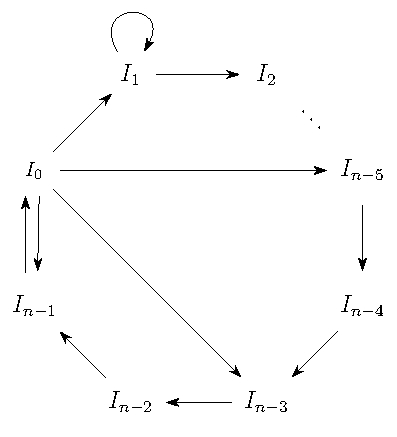
\includegraphics{images/graph_n.pdf}
% \caption[caption za v kazalo]{Dolg caption pod sliko}
  \caption[Primer vektorske slike.]{Relacije pokritja v trditvi~\ref{trd:pokritja} lahko prikažemo z grafom.}
  \label{fig:nkotnik}
\end{figure}

\begin{proof}[Dokaz trditve~\ref{trd:pokritja}]
Dokazovali bomo vsako točko posebej. 

Pri dokazu točke~\ref{trd:pokritja1} bomo dokazali še močnejšo trditev, ki nam bo v pomoč tudi pri dokazu druge točke. Pokazali bomo, da za vsak $j = 0, 1, \dots, n-1$ velja relacija pokritja $I_j \to I_1$.  Za dokaz je dovolj, če se prepričamo, da za vsak $j=0, 1, \dots, n-1$ množica $f(I_j)$ vsebuje točki $x_0$ in $x_1$. To je res, saj posledica~\ref{pos:vmesnavrednost} zagotavlja, da so v množici $f(I_j)$ vsebovane tudi vse točke iz intervala $(x_0, x_1)$. V primeru intervala $I_0 = [x_n, x_{n-2}]$ ugotovimo, da obe krajišči $I_0$ ležita na isti strani točke $c$. Lastnost \ref{eq:š4} pove, da krajišče $x_{n-2}$ menja strani, medtem ko lastnost~\ref{eq:š5} pravi, da točka $x_n$ ne menja strani, zato točki $f(x_n)$ in $f(x_{n-2})$ ležita na nasprotnih straneh točke $c$. V primeru intervala $I_j$ za $j = 1, 2, \dots, n-1$ iz lastnosti~\ref{eq:š2} izvemo, da krajišči intervala $I_j$ ležita na nasprotnih straneh točke $c$. Lastnost~\ref{eq:š4} pove, da obe krajišči menjata strani. Torej za vsak $j=0, 1, \dots, n-1$ interval $f(I_j)$ vsebuje točke cikla $\mathcal{O}$, ki ležijo na obeh straneh centra $c$. Zagotovo vsebuje točki $x_0$ in $x_1$ in zato tudi interval $I_1$.

Naj bo $j$ tako naravno število, za katerega velja $1 \leq j \leq n-1$. Želimo pokazati, da množica $f(I_j)$ vsebuje interval $I_{j+1}$. Vemo že, da interval $f(I_j)$ vsebuje točki $x_0$ in $x_1$. Za dokaz točke~\ref{trd:pokritja2} moramo pokazati samo še vsebovanost točke $x_{j+1}$ v množici $f(I_j)$. Podobno kot prej posledica~\ref{pos:vmesnavrednost} zagotavlja, da je v množici $f(I_j)$ vsebovan celoten interval $I_{j+1}$. V množici $f(I_j)$ so vsebovane točke $x_0, x_1$ in $f(x_j)$, zato je v tej množici vsebovana tudi množica točk $\mathcal{O}_{f(x_j)}$. Iz lastnosti~\ref{eq:š3} ugotovimo točka $x_{j+1}$ leži v množici $\mathcal{O}_{f(x_j)}$, zato velja $x_{j+1} \in \mathcal{O}_{f(x_j)} \subset f(I_j)$. Torej je interval $I_{j+1}$ res vsebovan v množici $f(I_j)$.

Za dokaz točke~\ref{trd:pokritja3} moramo pokazati, da je za vsako liho število $1 \leq l \leq n$ interval $I_{n-l}$ vsebovan v množici $f(I_0)$.  
Ker že vemo, da $f(I_0)$ vsebuje točki $x_0$ in $x_1$, preostane za dokazati še, da vsebuje točko $x_{n-l}$ Zaradi lastnosti~\ref{eq:š2} leži točka na drugi strani točke $c$ kot točki $x_{n-2}$ in $x_n$. Iz lastnoti~\ref{eq:š3} sklepamo, da je točka $x_{n-1}$ bolj oddaljena od točke $c$, kot točka $x_{n-l}$ za liho število $3 \leq l \leq n$ interval $I_{n-l}$, zato vsak interval, ki vsebuje točke $x_0, x_1$ in $x_{n-1}$, vsebuje tudi vse točko $x_{n-l}$ Pokazati moramo samo še, da množica $f(I_0)$ vsebuje točko $x_{n-1}$. Pri lastnosti~\ref{eq:š4} namesto $j$ pišemo $n-2$ in dobimo vsebovanost $x_{n-1} \in \mathcal{O}_{f(x_{n-2})}$. Interval $f(I_n)$ vsebuje točke $x_0, x_1$ in $f(x_j)$, 
\end{proof}


\begin{proof}[Dokaz trditve~\ref{trd:zap-cikel}]
Naj veljajo predpostavke v trditvi~\ref{trd:zap-cikel}. Radi bi pokazali, da ima funkcija $f$ za vsako naravno število $l\triangleleft m$ točko periode $l$. Dokaz bomo razdelili na tri dele. Najprej bomo dokazali izrek za liha števila manjša od $m$, potem za soda števila manjša od $m$ in na koncu še za vsa števila večja od $m$.
Pri dokazu si bomo pomagali z naslednjimi zankami, ki jih preberamo s slike~\ref{fig:nkotnik}:
\begin{enumerate}[label={(Z\arabic*)}]
\item $I_1 \to I_1$,\label{eq:z1}
\item$I_0\to I_{n-(l-1)} \to I_{n-(l-2)} \to \cdots \to I_{n-2} \to I_{n-1} \to I_0$ za sodo število $l \leq n$,\label{eq:z2}
\item $I_0\to\underbrace{I_1 \to I_1 \to \cdots  \to I_1}_{l - n +1 \text{ ponovitev intervala } I_1} \to I_2 \to \cdots \to I_{n-1} \to I_0 $ za $l \geq n$.\label{eq:z3}
\end{enumerate}
Edino liho število $l$ manjše od $m$, za katerega lahko velja $l\triangleleft m$ je število 1. Za $l=1$ uporabimo zanko~\ref{eq:z1}, ki je zanka dolžine 1 in zato elementarna. Torej obstaja točka periode 1 v intervalu $I_1$.

Naravno število  $1<l \leq m$ je lahko v relaciji $l \triangleleft m$ samo, če je sodo. Za vsako sodo število $l \leq n$ uporabimo zanko~\ref{eq:z2}.
Iz konstrukcije intervalov $I_0, I_1, \dots, I_n$ vemo, da je notranjost intervala $I_0$ disjunktna z intervali $I_{n-(l-1)}, I_{n-(l-2)}, \dots, I_{n-2}, I_{n-1}$. Krajišči intervala $I_0$ imata periodo $m$ in zato ne moreta sledit zanki~\ref{eq:z2}, katere dolžina je manjša od $m$. Z uporabo leme~\ref{lem:element} ugotovimo, da je zanka~\ref{eq:z2} elementarna, zato obstaja točka iz $I_0$, ki ima periodo $l$.

V primeru, ko je $l >n$, si pomagamo z $l$-zanko~\ref{eq:z3}.
Če je $l=m$, potem lahko izberemo poljubno točko iz cikla $\mathcal{O}$, saj imajo vse točke iz cikla $\mathcal{O}$ periodo $m$. Predpostavimo, da je $l \neq m$. Podobno kot v prejšnjem primeru je notranjost intervala $I_0$ disjunktna z intervali $I_1, I_2, \dots, I_{n-1}$. Pri dokazu, da kraišči intervala $I_0$ ne sledita zanki~\ref{eq:z3}, bomo obravnavali dva primera. Če velja $n<l<m$, potem krajišči intervala ne moreta slediti zanki~\ref{eq:z3}, saj je njena dolžina manjša od $m$, perioda krajišč intervala $I_0$ pa je $m$. Če je $l >m$ si pogledamo, koliko ponovitev intervala $I_1$ nastopa v zanki~\ref{eq:z3}. Število $l$ je večje od števila $m$. Iz opombe~\ref{op:štefzap} lahko preberemo, da je število $m$ večje od števila $n+1$ in naredimo naslednje ocene:
$$l-n+1>m-n+1 \geq n+1-n+1 = 2.$$
Število ponovitev intervala $I_1$ je večje od 2, kar pomeni, da se v zanki~\ref{eq:z3} interval $I_1$ pojavi vsaj trikrat. Ker za nobeno točko iz cikla $\mathcal{O}$ v intervalu $I_1$ ne ležijo tri zaporedne iteracije, tudi krajišča intervala $I_0$ ne morejo slediti zanki~\ref{eq:z3}. S pomočjo leme~\ref{lem:element} sklepamo, da je zanka~\ref{eq:z3} elementarna, kar zagotavlja obstoj točke iz intervala $I_0$, ki ima periodo $l$.
\end{proof}

Pri pozornem spremljanju dokaza opazimo, da smo dokazali močnejšo trditev.

\begin{trditev}\label{trd:posplositev}
Če $m$-cikel $\mathcal{O}$ vsebuje Štefanovo zaporedje dolžine $n<m-1$, potem ima obstaja periodična točka s periodo 1 (sledi iz zanke~\ref{eq:z1}), točka s sodo periodo $l \leq n$ (sledi iz zanke~\ref{eq:z2}) in točka s periodo $l \geq n$ (sledi iz zanke~\ref{eq:z3}).
\end{trditev}

S pomočjo trditve~\ref{trd:posplositev} lahko dokažemo tudi obstoj nekaterih periodo $l$, kjer je $l \triangleright m$. 
%Vsakič, ko iz $m$-cikla $\mathcal{O}$ izberemo $n+1$ točk, ki tvorijo štefanovo zaporedje 
Ekstremen primer dobimo, če je točka $q$ največja točka intervala $\mathcal{O}$ in točka $f(q)$ najmanjša točka intervala $\mathcal{O}$.  V tem imamo cikel oblike:
\tikz{
\tikzset{vertex/.style = {shape=circle, fill=black,draw,minimum size=3pt, inner sep=0pt}}
\tikzset{edge/.style = {->,> = latex'}}
	\node [vertex](1) at  (0, 0) {};
	\node (2) at (0.5, 0) {$\cdots$};
	\node[vertex] (3) at  (1, 0) {};
	\node[vertex] (4) at  (1.7, 0) {};
	\draw[edge, dashed] (3) to[bend left=20] (4);
	\draw[edge, dashed] (4) to[bend left=15] (1);
}.
Tri prikazane točke tvorijo Štefanovo zaporedje s tremi točkami, torej je $n=2$. Zaporedje zagotavlja obstoj periode 3 in zato obstoj vseh period.

%Dodatno onformacijo o prisotnosti periodičnih točk lahko dobimo tudi pri opazovanju ciklov dolžine $2^k$, za neko naravno število $k$. Če tak cikel vsebuje točko, ki ne menja strani, 


%#############  KONSTRUKCIJA ŠTEFANOVEGA ZAPOREDJA ##############
\section{Konstrukcija Štefanovega zaporedja} \label{konssz}
V tem poglavju bomo pokazali, da lahko v vsakem ciklu, ki vsebuje vsaj dve točki poiščemo Štefanovo zaporedje, razen če vsaka točka v ciklu menja stran. Dokaz bomo izvedli tako, da bomo konstruirali zaporedje in na koncu preverili, da gre za Štefanovo zaporedje.
\begin{trditev}
Cikel, ki vsebuje vsaj dve točki, vsebuje Štefanovo zaporedje, če vsaj ena točka ne menja strani.
\end{trditev}
\begin{proof}
Naj bo $m$ naravno število večje ali enako $2$ in naj bo $\mathcal{O}$ cikel sestavljen iz $m$ različnih točk. Naj bo množica $\mathcal{M}$ največji tak $\mathcal{O}$-interval, ki vsebuje točke $p, q$ in take točke iz cikla $\mathcal{O}$, ki menjajo strani. To pomeni, da za poljubno točko $x \in \mathcal{M} \cap \mathcal{O}$ vse točke iz množice $\mathcal{O}_x$ menjajo strani. Pri konstrukciji Štefanovega zaporedja, si bomo pomagali z množico $\mathcal{S} \subset \mathcal{O}$, ki vsebuje vse točke, ki so kandidati za nekončne člene Štefanovega zaporedja. V množici $\mathcal{S}$ ležijo take točke $x \in \mathcal{O} \cap \mathcal{M}$, ki jih funkcija $f$ slika dlje od točke $c$ kot katerokoli drugo točko iz množice $\mathcal{O}_x$ (slika~\ref{fig:S}). 
\begin{figure}[h]
  \centering
  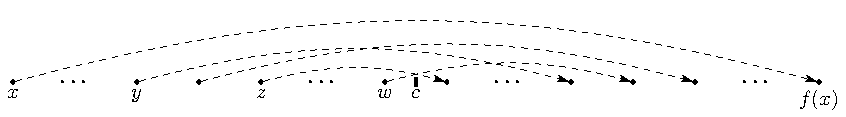
\includegraphics{images/mnozica_S.pdf}
% \caption[caption za v kazalo]{Dolg caption pod sliko}
  \caption[Konstrukcija množice S.]{Točka $x$ pripada množici $\mathcal{S}$, medtem ko točka $y$ pripada množici $\mathcal{M}$ ne pa tudi množici $\mathcal{S}$, saj se točka $z$ slika bolj stran od točke $c$ kot točka $y$.}
  \label{fig:S}
\end{figure}
Za vsak $x \in \mathcal{O} \cap \mathcal{M}$ velja, da je $x$ iz množice $\mathcal{S}$, če je $\mathcal{O}_{f(w)} \subset \mathcal{O}_{f(x)}$ za vsako točko $w \in \mathcal{O}_x$. Množica $\mathcal{S}$ zagotovo ni prazna množica, saj vsebuje točki $p$ in $q$. Sedaj lahko definiramo preslikavo $\sigma : \mathcal{S} \to \mathcal{O}$, ki slika element Štefanovega zaporedja v naslednji člen tega zaporedja. Za $\sigma(x)$ vedno izberemo točko iz množice $\mathcal{O}_{f(x)}$. Točka $x$ je vsebovana v množici $\mathcal{S}$, torej menja strani. To zagotavlja, da točki $x$ in $\sigma(x)$ ležita na nasprotnih straneh točke $c$. Točko $\sigma(x)$ določimo na naslednji način:
\begin{enumerate}[label={(\arabic*)}]
\item\label{def:sigma1} Če $f(x) \in \mathcal{M}$, potem je $\sigma(x)$ tista točke iz množice $\mathcal{O}_{f(x)}$, ki se s funkcijo $f$ slika najdlje od centra $c$. Velja vsebovanost:
$$f(\mathcal{O}_{f(x)}) \subseteq \mathcal{O}_{f(\sigma(x))}.$$
\item\label{def:sigma2} Če $f(x) \notin \mathcal{M}$, potem za $\sigma(x)$ izberemo katero koli točko iz $\mathcal{O}_{f(x)}$, ki ne menja strani.
\end{enumerate}
Iz definicije preslikave $\sigma$ vidimo, da v primeru~\ref{def:sigma1} točka $\sigma(x)$ leži v množici $\mathcal{S}$, saj menja strani in se slika bolj stran od točke $c$ kot katero koli drugo število iz množice $\mathcal{O}_{\sigma(x)}$. Primer si lahko pogledamo na sliki~\ref{fig:sigma}.
\begin{figure}[h]
  \centering
  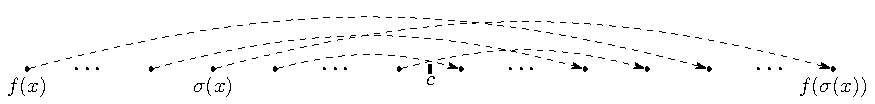
\includegraphics{images/sigma.pdf}
% \caption[caption za v kazalo]{Dolg caption pod sliko}
  \caption{Ker $f(x)$ menja strani, smo točko $\sigma(x)$ določili po primeru~\ref{def:sigma1}.}
  \label{fig:sigma}
\end{figure}

V primeru~\ref{def:sigma2} $\sigma(x)$ ne leži v množici $\mathcal{S}$, saj ne menja strani. Glede na to, da so v množici $\mathcal{S}$ kandidati za nekončne člene zaporedja, je $\sigma(x)$, ki ga dobimo v primeru~\ref{def:sigma2}, dober kandidat za končen člen zaporedja.

Števili $x$ in $\sigma(x)$ ležita na nasprotnih straneh točke $c$. Če je število $\sigma^2(x)$ dobro definirano, tudi števili $\sigma(x)$ in $\sigma^2(x)$ ležita na nasprotnih straneh točke $c$, kar pomeni, da točki $x$ in $\sigma^2(x)$ ležita na isti strani točke $c$. Kot smo utemeljili v poglavju~\ref{stefan_zap}, je za dokaz zelo pomembno, da se točke spiralno oddaljujejo od točke $c$, kot kaže slika~\ref{fig:spiral} in je podrobneje opisano v definiciji Štefanovega zaporedja v točkah~\ref{eq:š2} in~\ref{eq:š3}. Za vsako točko $x$ iz štefanovega zaporedja bi radi videli, da je $\sigma^2(x)$, če ta obstaja, bolj stran od točke $c$ kot točka $x$. Torej, $\sigma^2(x) \notin \mathcal{O}_x$.


\begin{lema}\label{lem:vtms}
Če obstaja taka točka $x \in \mathcal{S}$, za katero je $\sigma^2(x) \in \mathcal{O}_x$, potem vse točke cikla $\mathcal{O}$ menjajo stran.
\end{lema}
\begin{proof}
Denimo, da je za neko točko $x \in \mathcal{O}$ točka $\sigma^2(x)$ dobro definirana in da je vsebovana v množici $\mathcal{O}_x$. Potem so dobro definirane vse točke $x, y:=\sigma(x)$ in $z:=\sigma(y) = \sigma^2(x)$. Da lahko izračunamo $\sigma(x)$ ali $\sigma(y)$, morata točki $x$ in $y$ ležati v množici $\mathcal{S}$. Točka $y=\sigma(x)$ je izračunana po pravilu~\ref{def:sigma1} v definiciji preslikave $\sigma$, iz česar lahko sklepamo, da velja vsebovanost:
$$f(\mathcal{O}_{f(x)}) \subset \mathcal{O}_{f(\sigma(x))}=\mathcal{O}_{f(y)}.$$
Točka $x$ je vsebovana v množici $\mathcal{M}$, zato vse točke iz množice $\mathcal{O}_x$ menjajo strani. To pomeni, da točka $z = \sigma(y) \in \mathcal{O}$ menja strani in je izračunana po pravilu~\ref{def:sigma1} v definiciji preslikave $\sigma$. Torej tudi točka $z$ leži v množici $\mathcal{S}$ in velja vsebovanost:
$$f(\mathcal{O}_{f(y)}) \subset \mathcal{O}_{f(\sigma(y))}=\mathcal{O}_{f(z)}.$$
Iz dejstva, da točka $x$ pripada množici $\mathcal{S}$, sklepamo, da se $x$ s funkcijo $f$ slika dlje od centra $c$ kot katera koli druga točka iz množice $\mathcal{O}_x$. Točka $z=\sigma^2(x)$ pripada množici $\mathcal{O}_x$, zato točka $f(z)$ leži bližje centru kot točka $f(x)$, kar lahko zapišemo tudi tako:
$$\mathcal{O}_{f(z)} \subset \mathcal{O}_{f(x)}.$$
Ugotovili smo, da je slika množice $\mathcal{O}_{f(x)}$ vsebovana v množici $\mathcal{O}_{f(y)}$ in da je slika množice $\mathcal{O}_{f(y)}$ vsebovana v množici $\mathcal{O}_{f(x)}$. Ker točki $x$ in $y$ ležita na nasprotnih straneh točke $c$ in ker obe točki menjata strani, tudi točki $f(x)$ in $f(y)$ ležita na nasprotnih straneh točke $c$. Sklepamo lahko, da sta množici $\mathcal{O}_{f(x)}$ in $\mathcal{O}_{f(y)}$ disjunktni in ležita na nasprotnih straneh točke $c$. To pomeni, da vse točke iz množice $\mathcal{O}_{f(x)} \cup \mathcal{O}_{f(y)}$ menjajo strani. Množica $\mathcal{O}_{f(x)} \cup \mathcal{O}_{f(y)}$ je podmnožica cikla $\mathcal{O}$, ki se s funkcijo $f$ slika nazaj vase. Edina podmnožica cikla $\mathcal{O}$, ki se s $f$ slika nazaj vase, je množica $\mathcal{O}$, zato je cikel $\mathcal{O}$ enak uniji $\mathcal{O}_{f(x)} \cup \mathcal{O}_{f(y)}$. To pomeni, da vsaka točka iz cikla $\mathcal{O}$ menja strani. 
\end{proof}
Za dokončanje dokaza predpostavimo, da obstaja točka iz cikla $\mathcal{O}$, ki ne menja strani. Pokažimo, da potem obstaja Štefanovo zaporedje.
Če za implikacjo v lemi~\ref{lem:vtms} uporabimo pravilo kontrapozicije, dobimo naslednjo izjavo: Če obstaja točka iz cikla $\mathcal{O}$, ki ne menja strani, potem ne obstaja točka $x$, za katero velja $\sigma^2(x) \in \mathcal{O}_x$. To pomeni, da ne moreta biti hkrati izpoljneni enakosti $\sigma(p) = q$ in $\sigma(q) = p$. Lahko izberemo taki točki $x_0$ in $x_1$, da je $\{x_0, x_1\} = \{p, q\}$ in $x_2 := \sigma(x_1) \neq x_0$. Dokler je $x_i$ vsebovan v množici $\mathcal{S}$, dobimo naslednji člen s predpisom $x_{i+1} = \sigma(x_i)$.

Za dokončanje dokaza se moramo prepričati, da tako definirano zaporedje ustreza vsem petim pogojem iz definicije~\ref{def:stef}.
Zaradi izbire točk $\{x_0, x_1\} = \{p, q\}$ zaporedje ustreza pogoju~\ref{eq:š1}.
Točki $x_0$ in $x_1$ ležita na nasprotnih straneh točke $c$, ostale točke pa ležijo alternirajoče na levi oziroma desni strani točke $c$, saj zaporedni točki $x_i$ in $x_{i+1}=\sigma(x_i)$ ležita na nasprotnih straneh. S tem je izpolnjen pogoj~\ref{eq:š2}.
Za dokaz pogoja~\ref{eq:š3} se moramo prepričati, da se točke v zaporedju spiralno oddaljujejo od centra $c$. Začetne točke so bile izbrane tako, da točka $x_2$ ne leži v množici $\mathcal{O}_{x_0}$. Lema~\ref{lem:vtms} pokaže, da lahko podoben sklep naredimo tudi za ostale člene zaporedja, velja namreč $x_{i+2} = \sigma^2(x_i) \notin \mathcal{O}_{x_i}$. To pa pomeni, da število $x_{i+2}$ leži bolj stran od točke $c$ kot število $x_i$. Iz tega med drugim sledi, da so členi zaporedja paroma različni. Ker pa ležijo členi zaporedja v končni množici $\mathcal{O}$, obstaja končni člen tega zaporedja. Označimo ga z $x_n$.
Glede na definicijo zaporedja za vsako naravno število $j<n$ točka $x_j$ menja stran in velja $x_{j+1} = \sigma(x_j) \in \mathcal{O}_{f(x)}$. S tem je izpolnjen tudi pogoj~\ref{eq:š4}.
Za izpolnitev pogoja~\ref{eq:š5} se moramo prepričati, da zadnji člen $x_n$ ne menja strani. Število $x_n=\sigma(x_{n-1})$ smo dobili s predpisom~\ref{def:sigma2} v definiciji funkcije $\sigma$. Če točko $x_n$ določimo s pomočjo predpisa~\ref{def:sigma1}, potem $x_n$ leži v množici $\mathcal{S}$. Točka $x_n$ menja strani in se slika dlje od točke $c$ kot katera koli druga točka iz množice $\mathcal{O}_x$. Lahko izberemo točko $x_{n+1} = \sigma(x_n)$ in točka $x_n$ ni zadnja točka zaporedja, kar je protislovje s predpostavko, da je $x_n$ zadnja točka zaporedja. Točko $x_n$ smo zato dobili iz predpisa~\ref{def:sigma2}, kar pomeni, da $x_n$ ne menja strani. S tem je izpolnjena tudi zadnja zahteva~\ref{eq:š5} in je zaporedje $x_i$ res Štefanovo zaporedje. 
\end{proof}
V lemi~\ref{lem:vtms} smo ugotovili, da za naravno število $m \geq 2$ vsak $m$-cikel $\mathcal{O}$, ki vsebuje vsaj eno točko, ki ne menja strani, vsebuje Štefanovo zaporedje. V trditvi~\ref{trd:zap-cikel} pa smo se prepričali da cikli, ki vsebujejo Štefanovo zaporedje implicirajo obstoj elementarnih $\mathcal{O}$-vsiljenih $l$-zank za vsak $l\triangleleft m$. Dobimo naslednjo trditev: 

\begin{trditev}\label{trd:tnmsoc}
Naj bo $m$ naravno število večje od 2. Če $m$-cikel vsebuje točko, ki ne menja strani, potem za vsako naravno število $l$, za katero velja $l \triangleleft m$ obstaja elementarna $\mathcal{O}$-vsiljena $l$-zanka $\mathcal{O}$-intervalov in zato tudi točka s periodo $l$.
\end{trditev}
 %#############  DOKAZ IZREKA ŠARKOVSKEGA ##############
\section{Dokaz izreka Šarkovskega}
V tem poglavju bomo dokazali glavni del izreka Šarkovskega. Vemo že, da izrek velja, če obstaja točka cikla, ki ne menja strani. V primeru, da vse točke menjajo strani, bomo podobno kot v primeru~\ref{primer4} cikel razdelili na levo in desno polovico. Vsaka polovica tvori cikel za funkcijo $f^2$. Informacijo o ciklih funkcije $f^2$ bomo nato prenesli na cikle funkcije $f$.

\begin{trditev}\label{trd:realcvtm}
Naj bosta $m$ in $l$ naravni števili v relaciji $m \triangleright l$ in naj bo $\mathcal{O}$ $m$-cikel. Potem obstaja $\mathcal{O}$-vsiljena elementarna $l$-zanka $\mathcal{O}$-intervalov in posledično točka s periodo $l$.
\end{trditev}

\begin{proof}
%Vemo že, da dokaz velja, če cikel $\mathcal{O}$ vsebuje Štefanovo zaporedje. To se zgodi vsakič, ko vsaj ena točka cikla $\mathcal{O}$ menja stran. Trditev moramo dokazati še v primeru, ko vsaka točka cikla $\mathcal{O}$ menja stran. Predpostavimo, da je cikel $\mathcal{O}$ tak, da vsaka točka iz cikla menja stran. 
Izrek bomo dokazali s pomočjo indukcije na število $m$. 

Če je $m=1$, je trditev avtomatično izpolnjena, saj je 1 zadnji člen zaporedja Šarkovskega in edino število $l$, za katerega velja $l \triangleleft 1$ je 1. 

Predpostavimo, da izrek velja za vse cikle, katerih dolžina je krajša od $m$. Radi bi dokazali, da velja tudi za poljuben $m$-cikel $\mathcal{O}$. Če obstaja točka iz cikla $\mathcal{O}$, ki ne menja strani, potem je po trditvi~\ref{trd:tnmsoc} resična tudi trditev~\ref{trd:realcvtm}. V nasprotnem primeru vse točke cikla $\mathcal{O}$ menjajo strani. Označimo najmanjšo točko cikla $\mathcal{O}$  z $L$ in največjo točko cikla $\mathcal{O}$ z $R$. Množica $\mathcal{O}_L$ vsebuje vse točke iz cikla $\mathcal{O}$, ki ležijo levo od centra $c$, množica $\mathcal{O}_R$ pa vsebuje vse točke, ki ležijo desno od centra $c$. Ker vse točke iz cikla $\mathcal{O}$ menjajo strani, funkcija $f$ slika množico $\mathcal{O}_L$ v množico $\mathcal{O}_R$ in obratno. Funkcija $f|_{\mathcal{O}_L}$ je bijekcija iz množice $\mathcal{O}_L$ v množico $\mathcal{O}_R$ in funkcija $f|_{\mathcal{O}_R}$ je bijekcija iz množice $\mathcal{O}_R$ v množico $\mathcal{O}_L$. Ugotovimo, da množici $\mathcal{O}_L$ in $\mathcal{O}_R$ vsebujeta enako število točk, zato je število $m$ sodo in obstaja naravno število $n$, za katerega je $m = 2 n$. Ker je $m$ sodo število, je lahko neko naravno število $l$ v relaciji $l \triangleleft m$ samo, če je $l=1$ ali pa je $l$ sodo število. V drugem primeru obstaja tako naravno število $k$, za katerega je $l = 2 k$. Iz zgornjega razmisleka in iz trditve~\ref{trd:doubling} sledi, da je neko naravno število $l$ v relaciji $l \triangleleft m$ natanko tedaj, ko je $l=1$ ali pa je $l=2k$ in je število $k$ v relaciji $k \triangleleft n$. To pomeni, da moramo pokazati, da ima $f$ elementarno 1-zanko in elementarno $\mathcal{O}$-vsiljeno $2k$-zanko $\mathcal{O}$-intervalov za vsako naravno število $k$ za katerega velja relacija $k \triangleleft n$. Elementarno 1-zanko dobimo s pomočjo intervala $[p, q]$. Točka $p$ je največja točka množice $\mathcal{O}_L$ in točka $q$ je najmanjša točka množice $\mathcal{O}_R$. Ker točka $f(p)$ leži v množici $\mathcal{O}_R$ in točka $f(q)$ leži v množici $\mathcal{O}_L$ dobimo elementarno 1-zanko $[p, q] \to [p, q]$.
Pri dokazovanju obstoja $2k$-zanke za vsako naravno število $k$, ki ustreza relaciji $k \triangleleft n$, si bomo pomagali z indukcijsko predpostavko. Opazimo, da sta množici $\mathcal{O}_L$ in $\mathcal{O}_R$  cikla dolžine $n$ za funkcijo $f^2$. Ker je dolžina obeh ciklov manjša od $m$, lahko uporabimo indukcijsko predpostavko. Če indukcijsko predpostavko uporabimo na ciklu $\mathcal{O}_R$, ugotovimo, da za vsako naravno število $k$, za katerega je $k \triangleleft n$, obstaja elementarna $\mathcal{O}_R$-vsiljena $k$-zanka $\mathcal{O}_R$ intervalov za funkcijo $f^2$. Pokazati moramo, da te zanke zagotavljajo obstoj elementarnih $l$-zank za funkcijo $f$. Poglejmo si poljubno elementarno $k$-zanko $\mathcal{O}_R$ intervalov za funkcijo $f^2$:
\begin{equation}\label{kloop}
I_0 \xrightarrow{f^2} I_1 \xrightarrow{f^2} I_2 \xrightarrow{f^2} \cdots \xrightarrow{f^2} I_{k-1} \xrightarrow{f^2} I_0.
\end{equation}
Za vsako naravno število $0 \leq i < k$ označimo najkrajši zaprti interval, ki vsebuje množico $f(I_i \cap \mathcal{O}) \subset \mathcal{O}_L$, z $I_i'$. Intervali $I_i'$ so $\mathcal{O}$-intervali za katere veljajo relacije pokritja $I_i \xrightarrow{f} I_i'$. Če interval $I_0$ označimo z $I_k$ lahko naradimo naslednji razmislek. Za vsako naravno število $0 \leq i < k$ lahko zapišemo $\mathcal{O}_R$-vsiljene relacije pokritja $I_i \xrightarrow{f^2} I_{i+1}$, zato obstajata taki točki $a_i, b_i \in I_i \cap \mathcal{O}_R$, da interval $I_{i+1}$ leži v intervalu omejenim s točkama $f^2(a_i)$ in $f^2(b_i)$. Točki $a_i' := f(a_i)$ in $b_i' := f(b_i)$ ležita v množici $I_i' \cap \mathcal{O}$ in zaprt interval omejen s točkama $f(a_i') = f^2(a_i)$ in $f(b_i') = f^2(b_i)$ vsebuje interval $I_{i+1}$. Dobili smo $\mathcal{O}$ vsiljeno relacijo pokritja $I_i' \xrightarrow{f} I_{i+1}$. S pomočjo zgornjih relacij pokritja lahko zapišemo naslednjo $\mathcal{O}$-vsiljeno $l$-zanko:
\begin{equation}\label{lloop}
I_0 \xrightarrow{f} I'_0 \xrightarrow{f} I_1 \xrightarrow{f} I'_1 \xrightarrow{f} \cdots \xrightarrow{f} I_{k-1} \xrightarrow{f} I'_{k-1} \xrightarrow{f} I_0
\end{equation}
Prepričajmo se, da je zanka~\eqref{lloop} elementarna. Naj bo točka $x$ periodična točka za funkcijo $f$, ki sledi zanki~\eqref{lloop}. Točka $x$ je periodična točka za funkcijo $f^2$, ki sledi zanki~\eqref{kloop}. Torej, točka $x$ ima periodo $k$ za funkcijo $f^2$, kar pomeni, da $k$ točk $f$-orbite leži v množici $\mathcal{O}_R$. Ker intervali v zanki~\eqref{lloop} ležijo izmenično na levi oziroma desni strani točke $c$, tudi iteracije točke $x$ ležijo izmenično na levi oziroma desni strani točke $c$. To pomeni, da $k$ točk, ki predstavljajo lihe iteracije točke $x$ ležijo v množici $\mathcal{O}_L$. Zato orbita točke $x$ vsebuje $2k = l$ različnih točk in je tudi perioda točke $x$ za funkcijo $f$ enaka $l$. Sklepamo, da je zanka~\eqref{lloop} elementarna, kar zakluči dokaz.
\end{proof}

%#############  REALIZACIJSKI IZREK ŠARKOVSKEGA ##############
\section{Dokaz realizacijskega izrek Šarkovskega}\label{sec:realizacija}
Daljši in bolj zapleten del dokaza izreka Šarkovskega je za nami. Sedaj moramo dokazati še drugi del, ki pravi:
\begin{izrek}
Vsak rep $\mathcal{T}$ ureditve Šarkovskega je množica period za neko zvezno funkcijo $f$, ki slika interval nazaj vase.
\end{izrek}
\begin{proof}
Izrek bomo dokazali tako, da bomo za vsak rep $\mathcal{T}$ poiskali funkcijo, katere množica period je enaka repu $\mathcal{T}$. Pri iskanju primerne funkcije si bomo pomagali z družino odrezanih šotorskih funkcij:
\begin{equation*} %\label{eq1}
\begin{split}
T_h &:  [0, 1] \to [0, 1] \\ 
T_h &: x \mapsto \min \left(h, 1- 2 \left|x-\frac{1}{2} \right|\right)
\end{split}
\end{equation*}
Ekvivalentno in mogoče lažje predstavljivo lahko predpis funkcije $T_h$ zapišemo na naslednji način:
\begin{equation*} %\label{eq1}
T_h(x) = \min(2x, 2-2x, h).
\end{equation*}
Točke, ki imajo za funkcijo $T_h$ periodo $n$, so negibne točke za funkcijo $T_h^n$, zato si lahko zaradi lažje predstave na sliki~\ref{fig:Th} ogledamo funkcije $T_{0,85}, T_{0,85}^2, T_{0,85}^3$ in $T_{0,85}^4$. 
\begin{figure}[h]
  \centering
  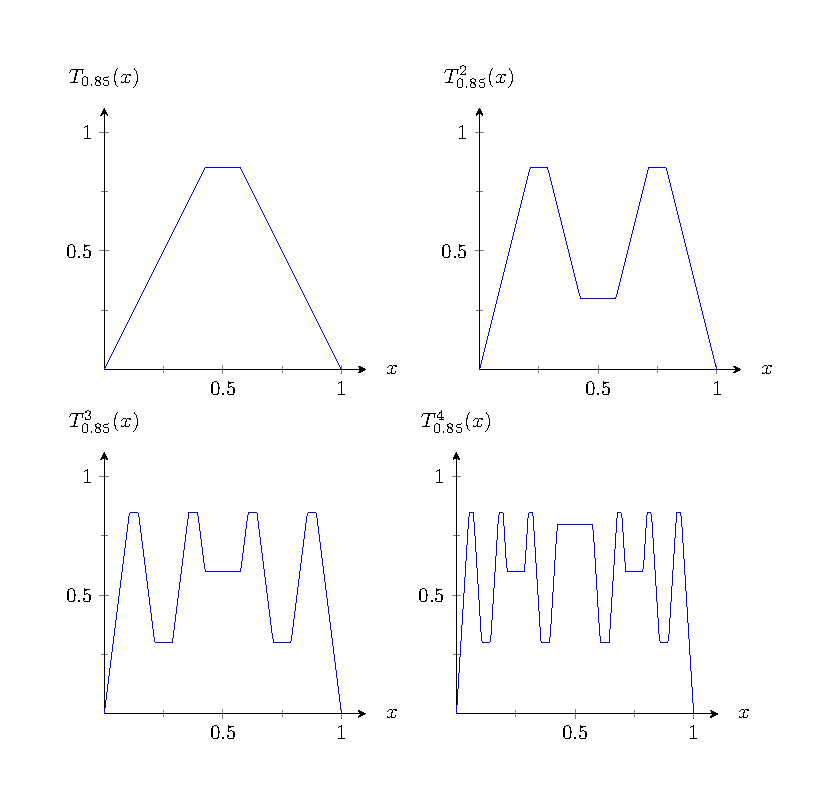
\includegraphics{images/odrezana_funkcija.pdf}
% \caption[caption za v kazalo]{Dolg caption pod sliko}
  \caption[Primer vektorske slike.]{Funkcije  $T_{0,85}, T_{0,85}^2, T_{0,85}^3$ in $T_{0,85}^4$ in njihova presečišča s simetralo lihih kvadrantov.}
  \label{fig:Th}
\end{figure}

Pri dokazu bo zelo pomembna funkcija $T_1$. Na sliki~\ref{fig:T1} so prikazane prve štiri iteracije funkcije $T_1$. Iz slike preberemo, da ima funkcija $T_1$ dve presečišči s simetralo lihih kvadrantov in zato tudi dve negibni točki. Funkcija $T_1^2$ ima 4 negibne točke, funkcija $T_1^3$ jih ima 8, funkcija $T_1^4$ pa 16. Opazimo, da funkcija $T_1^n$ seka simetralo lihih kvadrantov natanko $2^n$-krat in ima prav toliko negibnih točk. Funkcija $T_1$ pa ima po tem razmisleku največ $2^n$ točk s periodo $n$.
\begin{figure}[h]
  \centering
  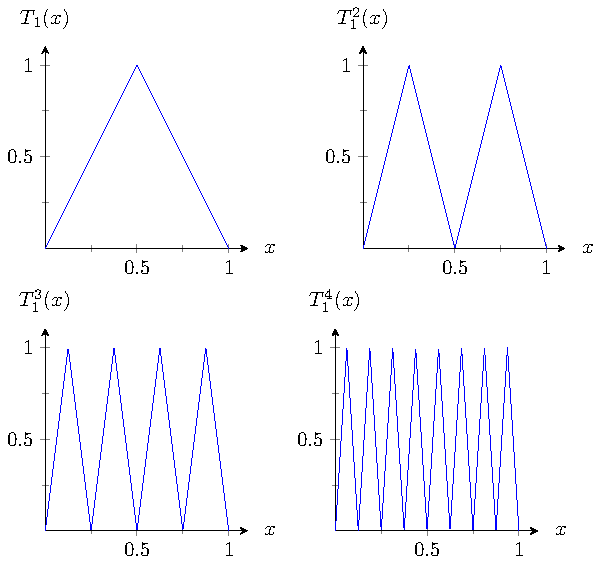
\includegraphics{images/funkcija_T1.pdf}
% \caption[caption za v kazalo]{Dolg caption pod sliko}
  \caption[Primer vektorske slike.]{Funkcije $T_1, T_1^2, T_1^3, T_1^4$ in njihova presečišča s simetralo lihih kvadrantov.}
  \label{fig:T1}
\end{figure}

Za dokaz izreka bomo najprej pokazali, da obstaja funkcija, ki ima samo periodo 1. To je funkcija $T_0$. Za vsak $x \in [0, 1]$ je vrednost funkcije $T_0$ enaka 0, zato je 0 tudi edina periodična točka za to funkcijo. Točka 0 je negibna točka, zato je njena perioda enaka 1.

Obravnavajmo funkcijo $T_1$. Dokazali bomo, da je vsako naravno število $n$ perioda funkcije $T_1$. To najlažje dokažemo tako, da poiščemo cikel dolžine 3 in s pomočjo izreka~\ref{izr:forcing} sklepamo, da ima funkcija $T_1$ vse periode. Vsaka točka ki ima za funkcijo $T_1$ periodo 3 je negibna točka funkcije $T_1^3$, zato si poglejmo negibne točke funkcije $T_1^3$. Iz grafa razberemo, da ima funkcija $T_1^3$ osem negibnih točk. Izračunamo lahko, da sta točki 0 in $\frac{2}{3}$ sta negibni točki funkcije $T_1$, točke $\frac{2}{7}, \frac{4}{7}$ in $\frac{6}{7}$ tvorijo 3-cikel. Prav tako tvorijo 3-cikel točke  $\frac{2}{9}, \frac{4}{9}$ in $\frac{8}{9}$. S pomočjo izreka~\ref{izr:forcing} ugotovimo, da funkcija $T_1$ vsebuje točke vseh period, saj vsebuje točko periode 3.

Funkciji $T_1$ in $T_h$ sta vsaj na nekem delu intervala $[0, 1]$ enaki, zato pričakujemo, da obstajajo cikli, ki so skupni obema funkcijama. O tem govori naslednja lema:
\begin{lema}\label{lem:t1th}
Za funkciji $T_1$, $T_h$ in njune cikle  veljata naslednji dve trditvi:
\begin{enumerate}[label={(\arabic*)}]
\item Če je $\mathcal{O} \subseteq [0, h]$ cikel za funkcijo $T_1$, je tudi cikel za funkcijo $T_h$. \label{trd:t1toth}
\item Če je $\mathcal{O} \subseteq [0, h)$ cikel za funkcijo $T_h$, je cikel tudi za funkcijo $T_1$. \label{trd:thtot1}
\end{enumerate}
\end{lema}
\begin{proof}
Funkciji $T_1$ in $T_h$ se razlikujeta samo v tistih točkah $x$, za katere je $T_1(x) > h$. V vseh ostalih točkah, sta funkciji enaki. Privzemimo, da je $\mathcal{O} \subset [0, h]$ cikel za funkcijo $T_1$. Ker je cikel $\mathcal{O}$ vsebovan v intervalu $[0, h]$, za vsako točko $x \in \mathcal{O}$ velja $T_1(x) \leq h$. Torej velja $T_1(x)=T_h(x)$, kar pomeni, da je $\mathcal{O}$ tudi cikel za funkcijo $T_h$. Dokazali smo trditev~\ref{trd:t1toth}

Za dokaz trditve~\ref{trd:thtot1} prespostavimo, da je $\mathcal{O} \subset [0, h)$ cikel za funkcijo $T_h$. Torej je za vsako točko $x$ iz cikla $\mathcal{O}$ slika $T_h(x)$ manjša od $h$. Velja, da je tudi vrednost $T_1(x)$ manjša od $h$. To pomeni, da sta vrednosti funkcij $T_1$ in $T_h$ v $x$ enaki. Ker to velja za vsako točko cikla $\mathcal{O}$, je $\mathcal{O}$ tudi cikel za funkcijo $T_1$.
\end{proof}
V trditvi~\ref{trd:thtot1} polodprtega intervala $[0, h)$ ne moremo zamenjati z zaprtim intervalom $[0, h]$, saj ne moremo narediti sklepa, da iz neenakosti $T_h(x) \leq h$ sledi neenakost $T_1(x) \leq h$. Za primer si lahko pogledamo funkcijo $T_{\frac{1}{2}}$, ki ima negibno točko $\frac{1}{2}$ na intervalu $[0, \frac{1}{2}]$, vendar to ni negibna točka funkcije $T_1$.
%\begin{primer}
%Za primer preučimo funkcijo $T_{0.88}$. Presečišča funkcije $T_{0,88}^3$ s simetralo lihih kvadrantov predstavljajo kandidate za periodične funkcije. Iz slike razberemo presečišče $(\frac{6}{25}, \frac{6}{25})$, kar pomeni, da je točka $\frac{6}{25}$ periodična točka za funkcijo $T_{0,88}$. Z iteracijami funkcije $T_{0,88}$ na točki $\frac{6}{25}$ dobimo 3-cikel $\mathcal{O} = \left\{ \frac{6}{25}, \frac{12}{25}, \frac{22}{25} \right\}$. Iz grafa funkcije $T_1^3$ vidimo, da točka $\frac{6}{25}$ ni fiksna točka funkcije $T_1^3$ in zato ne more biti točka periode 3 za funkcijo $T_1$. Cikel $\mathcal{O}$ res ni cikel za funkcijo $T_1$.
%\end{primer}
Ključna ideja tega dokaza je, da definiramo funkcijo $h(\cdot)$:
$$h: \N \to [0, 1], h(m) := \min\{\max \mathcal{O}: \mathcal{O}\text{ je }m\text{-cikel funkcije }T_1 \}$$
Prepričati se moramo, da je definicija dobra. Očitno je, da maksimum $m$-cikla obstaja. Pokazati moramo še, da obstaja tudi minimum. Funkcija $T_1^n$ seka simatralo lihih kvadratov $2^n$-krat, kar pomeni, da ima funkcija $T_1^n$ natanko $2^n$ negibnih točk, funkcija $T_1$ pa ima $2^n$ periodičnih točk. Ker je nabor točk končen, minimum obstaja.

Zvitost dokaza se skriva v tem, da pri funkciji $T_{h(m)}$ število $h(m)$ igra tri vloge. Pojavi se kot parameter, ki določi funkcijo iz družine funkcij. Predstavlja maksimum funkcije $T_{h(m)}$ in največjo točko neke orbite za funkcijo $T_{h(m)}$. Pokazali bomo, da funkcija $h(m)$ razvrsti naravna števila na interval $[0, 1]$ natančno v obratnem vrstnem redu, kot ureditev Šarkovskega.
Funkcija $h(\cdot)$ ima naslednje lastnosti:
\begin{enumerate}[(a)]
\item funkcija $T_h$  vsebuje $l$-cikel $\mathcal{O}\subset [0, h)$, če in samo če je $h(l)<h$,\label{l1}
\item orbita točke $h(m)$ je $m$-cikel za funkcijo $T_{h(m)}$,\label{l2}
\item vsi ostali cikli za funkcijo $T_{h(m)}$ ležijo v intervalu $[0, h(m)).$\label{l3}
\end{enumerate}

Lastnost~\ref{l1} je očitna iz definicije funkcije $h(\cdot)$.
%Prva lastnost sledi iz definicije funkcije $h(\cdot)$. Če funkcija $T_h$ vsebuje cikel $\mathcal{O}\subset [0, h)$, potem je največje točka tega cikla manjša od $h$, kar pomeni, da je točka $h(l)$ manjša od $h$. Obratno,Če je točka $h(l)$ manjša od $h$, potem $l$-cikel za funkcijo $T_h$, ki vsebuje točko $h(l)$ cel leži v intervalu $[0, h)$

Za dokaz lastnosti~\ref{l2} opazimo, da je točka $h(m)$ največja točka $m$-cilka $\mathcal{O}$ za funkcijo $T_1$, zato cikel $\mathcal{O}$ leži v intervalu $[0, h(m)]$. Po trditvi~\ref{trd:t1toth} iz leme~\ref{lem:t1th} je $\mathcal{O}$ cikel za funkcijo $T_{h(m)}$. 

Ker je $h(m)$ maksimum funkcije $T_{h(m)}$m vsi ostali cikli funkcije $T_{h(m)}$ ležijo v intervalu $[0, h)$. Pokazali smo lastnost~\ref{l3}

S pomočjo lastnosti~\ref{l1},~\ref{l2},~\ref{l3} in izreka~\ref{izr:forcing} lahko dokažemo naslednjo lemo, s pomočjo katere zaključimo dokaz realizacijskega izreka Šarkovskega.

\begin{lema}\label{lem:<rel}
Za poljubni naravni števili $m$ in $n$ velja ekvivalenca:
$$ n \triangleleft m \iff h(n) < h(m).$$
\end{lema}
\begin{proof}
Najprej pokažimo implikacijo v desno. Denimo, da sta števili $m$ in $l$ v relaciji $l \triangleleft m$. Zaradi lastnosti~\ref{l2} ima funkcija $T_h(m)$ $m$-cikel. Izrek~\ref{izr:forcing} zagotavlja, da ima funkcija $T_{h(m)}$ tudi cikel dolžine $l$. Iz lastnosti~\ref{l3} ugotovimo, da ta cikel leži v intervalu $[0, h(m))$. Na koncu upoštevamo še lastnost~\ref{l1} in se prepričamo, da je $h(l) < h(m)$

Pri dokazu implikacije v levo stran uporabimo pravilo kontrapozicije in dokazujemo izjavo: $ m \triangleleft l \iff h(m) < h(l)$. Zaradi simetričnosti števil $l$ in $m$ je ta izjava ekvivalentna prejšnji.
\end{proof}
Poglejmo, katere periode ima funkcija $T_{h(m)}$. Iz definicije funkcije $h(m)$ sledi, da je m perioda za funkcijo $T_{h(m)}$. Radi bi videli, da ima funkcija $T_{h(m)}$ periodo $l$ natanko tedaj, ko velja $l \triangleleft m$. Naj bo $l$ naravno število, za katerega velja relacija $l \triangleleft m$. Lema~\ref{lem:<rel} pravi, da velja neenakost $h(l) < h(m)$. Iz lastnosti~\ref{l1} sklepamo, da funkcija $T_{h(m)}$ vsebuje $l$-cikel. Sedaj predpostavimo, da funkcija $T_{h(m)}$ vsebuje $l$ cikel. Iz lastnosti~\ref{l1} sklepamo, da je $h(l) < h(m)$. Lema zagotavlja, da v tem primeru število $l$ zadošča relaciji $l \triangleleft m$. Torej je množica period za funkcijo $T_{h(m)}$ res množica $\{n \in \N; n \triangleleft m\}$.

Poiskati moramo še zvezno funkcijo ki ima za množico period množico vseh potenc števila 2. Definiramo $h(2^{\infty}) := \sup_k h(2^k)$. Za vsako naravno število $k$ velja $h(2^k) < h(2^{\infty})$. Zaradi lastnosti~\ref{l1} funkcija $T_{h(2^{\infty})}$ vsebuje $2^k$-cikel, za vsak $k \in \N$. 
Denimo, da funkcija $T_{h(2^{\infty})}$ vsebuje nek $m$ cikel, kjer število $m$ ni potenca števila 2. Zaradi izreka~\ref{izr:forcing} funkcija $T_{h(2^{\infty})}$ vsebuje tudi $2m$-cikel. Ker sta $m$-cikel in $2m$-cikil disjunktca, lastnost~\ref{l3} zagotavlja, da vsaj en od teh dveh ciklov leži v intervalu $[0, h(2^{\infty}))$. Recimo, da je to $m$-cikel. Potem obstaja tako naravno število $l$, da velja $h(m) < h(2^l)$. S pomočjo leme~\ref{lem:<rel} ugotovimo, da velja $m \triangleleft 2^l$, torej je število $m$ potenca števila 2. To je protislovje. Če bi predpostavili, da $2m$-cikel leži v intervalu $[0, h(2^{\infty}))$, bi prišli do sklepa, da je število $2m$ potenca števila 2, kar pa tudi vodi v protislovje. Funkcija $T_{h(2^{\infty})}$ res vsebuje samo cikle, katerih dolžina je potenca števila 2.

Za konec pokažimo, da obstaja funkcija, ki nima periodičnih točk. Za primer lahko vzamemo translacijo $f : \R \to \R$ s predpisom $f(x) = x + a$, kjer je $a$ katerokoli neničelno realno število.
\end{proof}


%#############  PROSTOR ŠARKOVSKEGA ##############
\section{Prostor Šarkovskega}
Po zaklučenem dokazu si radoveden matematik hitro postavi vprašanje, kako se spremenijo posledice v izreku, če spremenimo predpostavke izreka. Glede na to, kako spremenimo predpostavke, lahko pridemo do različnih posplošitev izreka. Tudi v primeru izreka Šarkovskega obstaja več posplošitev. Nekatere obravnavajo izrek tudi za nezvezne funkcije, ki ustrezajo določenim pogojem. Izrek Šarkovskega govori samo o zveznih funkcijah definiranih na intervalu, obstajajo pa posplošitve izreka, ki preučujejo zvezne funkcije, ki so definirane na drugih topoloških prostorih. Vprašamo se lahko, kakšna ureditev naravnih števil, če ta obstaja, opiše prisotnost periodičnih točk zvezne funkcije $f:X \to X$. Natančneje, iščemo relacijo $\triangleleft_X$ z lastnostjo: če je $m$ perioda za zvezno funkcijo $f:X \to X$, potem je vsako naravno število $l$, za katero je $l \triangleleft_X m$, tudi perioda za funkcijo $f$. Če je relacija $\triangleleft_X$ enaka relaciji Šarkovskega, ki smo jo spoznali v definiciji~\ref{def:ureditev-sark}, pravimo, da je prostor $X$ prostor Šarkovskega. To poglavje bomo namenili temu, da bomo spoznali nekaj prostorov Šarkovskega in tudi nekaj prostorov, ki to niso. Predstavili bomo tudi kakšno lastnost, ki jo imajo vsi prostori Šarkovskega. 

Najbolj tipični predstavniki prostorov Šarkovskega, so množica realnih števil in intervali v realnih številih. Poglejmo si primer prostora, ki ni prostor Šarkovskega.

\begin{primer}
Krožnica $S^1 = \{ (cos(\varphi), \sin(\varphi)), \varphi \in [0, 1) \}$ ni prostor Šarkovskega. Hitro se lahko prepričamo, da obstajajo funkcije, ki imajo samo eno periodo. To so rotacije okoli koordinatnega izhodišča. Definiramo družino funkciji: 
\begin{equation*} %\label{eq1}
\begin{split}
R_n &: S^1 \to S^1 \\ 
R_n &: (cos(\varphi), \sin(\varphi)) \mapsto (cos(\varphi + \frac{2 \pi}{n}), \sin(\varphi + \frac{2 \pi}{n})).
\end{split}
\end{equation*}
Vse točke iz krožnice $S^1$ so periodične točke za funkcijo $R_n$ in vse imajo periodo $n$. Zato iz obstoja periodične točke za zvezno funkcijo $f : S^1 \to S^1$ ne moremo sklepati na obstoj drugih period za to funkcijo.
\end{primer}
S podobnim sklepanjem kot zgoraj lahko hitro poiščemo veliko prostorov, ki niso prostori Šarkovskega. To naredimo tako, da poiščemo prostore, ki imajo kakšno os rotacijske simetrije in preverimo, da res niso prostori Šarkovskega. Primeri takih prostorov so npr. sfera, krogla, torus, piramida, kocka\dots 

Videli smo, da pri krožnici ne obstaja taka relacija, ki bi opisala periode zveznih funkcij iz prostora $S^1$ nazaj v prostor $S^1$. V naslednjem primeru bomo spoznali prostor, ki ni prostor Šarkovskega, vseeno pa lahko iz prisotnosti nekaterih period sklepamo na prisotnost durgih.
\begin{primer}
Naj bo prostor $X$ unija dveh disjunktnih intervalov: $X = [-2, -1] \cup [1, 2]$. Funkcija $g : X \to X$ podana s predpisom $g(x) = -x$ je zvezna funkcja. Vsaka točka iz prostora $X$ ima periodo 2, funkcija pa nima nobene fiksne točke, zato prostor $X$ ni prostor Šarkovskega. Vseeno pa lahko poiščemo relacijo $\triangleleft_X$, ki opiše katere periode ima lahko funkcija. Zaradi lažje obravnave bomo interval $[-2, -1]$ označili z $I_1$, interval $[1, 2]$ ia z $I_2$. Pri poljubni funkciji $f: X \to X$ imamo štiri možnosti. Če je $f(I_1) \subset I_1$ in $f(I_2) \subset I_2$ lahko za funkciji $f|_{I_1}$ in $f|_{I_2}$ uporabimo izrek Šarkovskega in ugotovimo, de je relacija $\triangleleft_X$ enaka relaciji Šarkovskega. V primeru, ko je $f(I_1) \subset I_1$ in $f(I_2) \subset I_1$ lahko periodične točke ležijo samo v intervalu $I_1$. Za funkcijo $f|_{I_1}$ uporabimo izrek Šarkovskega in ugotovimo, da je relacija $\triangleleft_X$ enaka relaciji Šarkovskega. Podoben sklep lahko naredimo tudi v primeru, ko je $f(I_1) \subset I_2$ in $f(I_2) \subset I_2$. Do spremembe pride, ko obravnavamo primer $f(I_1) \subset I_2$ in $f(I_2) \subset I_1$. V tem primeru se točke iz intervala $I_1$ s funkcijo $f$ slikajo v interval $I_2$ in obratno. Zato ima vsaka periodična točka sodo periodo. Naj bo $x \in X$ točks periode $2m$ za funkcijo $f$. Brez izgube splošnosti lahko sklepamo, da točka $x$ pripada intervalu $I_1$. Potem ima točka $x$ periodo $m$ za funkcijo $f^2|_{I_1} :I_1 \to I_1$. Ker je $I_1$ prostor Šarkovskega in je $f^2$ zvezna funkcija, lahko uporabimo izrek Šarkovskega in ugotovimo, da za vsako naravno število $l$, za katerega velja $l \triangleleft m$, obstaja točke $y \in I_1$ s periodo $l$ za funkcijo $f^2$. Točka $y$ ima periodo $2l$ za funkcijo $f$, saj $l$ je orbita točke $y$ sestavljen iz $l$ različnih točk v intervalu $I_1$ (sode iteracije) in $l$ različnih točk iz intervala $I_2$ (lihe iteracije). Ugotovili smo naslednje: Če ima zvezna funkcija $f:X \to X$ liho periodo $m$, potem ima zagotovo tudi vse periode $l$, kjer je $l \triangleleft m$. Če pa je perioda $m$ soda, potem ima funkcija vse periode $l=1$, za katere je $l \triangleleft m$.
Dobimo relacijo $\triangleright_X$:
$$3 \triangleright_X 5 \triangleright_X 7 \triangleright_X \cdots \triangleright_X 2\cdot 3 \triangleright_X 2\cdot 5 \triangleright_X 2\cdot 7 \triangleright_X \cdots \triangleright_X 2^2\cdot 3 \triangleright_X 2^2\cdot 5 \triangleright_X 2^2\cdot 7 \triangleright_X \cdots \triangleright_X 2^3 \triangleright_X 2^2 \triangleright_X 2.$$
$$3 \triangleright_X 5 \triangleright_X 7 \triangleright_X \cdots \triangleright_X 1.$$
\end{primer}

Na začetku primera smo enostavno pokazali, da disjunktna unija ni prostor Šarkovskega. Z zelo podobno idejo lahko pokažemo, da noben nepovezan prostor ni prostor Šarkovskega.

\begin{trditev}
Prostor Šarkovskega je povezan.
\end{trditev}
\begin{proof}
Naj bo prostor $X$ disjunktna unija prostorov $A$ in $B$ in naj bosta $a \in A$ in $b \in B$ poljubni točki tega prostora. Definiramo funkcijo $f:X \to X$ s predpisom:
\[ f(x) = \begin{cases}
  a, & \mbox{ če $x \in B $}\\
  b ,& \mbox{ če $x \in A$.}
  \end{cases}
  \]
Funkcija $f$ ima samo dve periodični točki. To sta točki $a$ in $b$. Obe pa imata periodo 2. Ker nobena točka prostora $X$ ni fiksna točka za funkcijo $f$, prostor $X$ ni prostor Šarkovskega.
\end{proof}

\begin{trditev}
Lastnost biti prostor Šarkovskega je topološka lastnost. To pomeni, če je $X$ prostor Šarkovskega in je prostor $Y$ homeomorfen prostoru $X$, potem je tudi $Y$ prostor Šarkovskega.
\end{trditev}
\begin{proof}
Naj bo prostor $X$ prostor Šarkovskega in naj bo prostor $Y$ homeomorfen prostoru $X$. Naj bo $h : X \to Y$ homeomorfizem med njima. Funkciji $f : Y \to Y$ in $g = h^{-1} \circ f \circ h : X \to X$ imata enake periode, zato je $Y$ tudi prostor Šarkovskega.
\end{proof}

\begin{definicija}
Naj bo $X$ topološki prostor in $A \subset X$ njegov podprostor. Preslikavi $r : X \to A$ pravimo \emph{retrakcija}, če je preslikava $r|_A = id_A$. Podprostor $A \subset X$ je \emph{retrakt} prostora $X$, če obstaja retrakcija $r: X \to A$.
\end{definicija}

\begin{trditev}
Retrakt prostora Šarkovskega je prostor Šarkovskega.
\end{trditev}
\begin{proof}
Denimo, da je prostor $X$ prostor Šarkovskega in prostor $A \subset X$ retrakt prostora $X$. Naj bo $r : X \to A$ retrakcija $i : X \to A$ inkluzija. Če je funkcija $f : A \to A$ zvezna, ima funkcija $g = i \circ f \circ r : X \to X$ enake periodične točke, kot funkcija $f$. Zato je prostor $A$ tudi prostor Šarkovskega.
\end{proof}


\begin{definicija}
Naj bo C grapf funkcije $\sin\left(\frac{1}{x}\right)$ na intervalu $x \in (0 , 1]$ in naj bo $A$ daljica $\{ 0 \} \times [-1 , 1]$. Varšavski lok je prostor $X = C \cup A$.
Prostor $X$ je kompakten in ima dve komponenti za povezavost s potmi. Komponenta $A$ je homeomorfna zaprtemu intervalu, komponenta $C$ pa je homeomorfna polodprtemu intervalu. Prostor je prikazan na sliki~\ref{fig:varsavski_lok}
\end{definicija}

\begin{trditev}
Varšavski lok je prostor Šarkovskega.
\end{trditev}
\begin{proof}
Varšavski lok zapišimo kot $X = C \cup A$, kjer je C krivulja $\{(x, \sin(\frac{1}{x})), x\in [0, 1]\}$ in $A= \{0\} \times [0, 1]$. Naj bo $x \in X$ točka s periodo $n$ in naj za neko naravno število $m$ velja relacija $m \triangleleft n$. Pokazali bomo, da obstaja točka $y$ s periodo $m$. Ker je funkcija $f$ zvezna, se ne more zgoditi, da ja $f(A) \subset C$ in $f(C) \subset A$. V tem primeru bi bila množica $f(C)$ kompaktna množica, ki je nima skupne točke z množico $C$. Ker ima prostor $\R$ lastnost $T_4$, obstajata disjunktni odprti množici, $U$ in $V$, za kateri velje $f(C) \subset U$, $f(A) \subset C \subset V$, kar predstavlja separacijo prostora $f(X)$, kar pa ni mogoče, saj Če je $f(A) \subset C$, potem je zaradi zveznosti funkcije $f$ tudi $f(C) \subset C$. Ker je $X$ kompaktna množica in je slika kompaktne množice z zvezno preslikavo kompaktna, je množica $f(X)$ kompaktna povezana podmnožica množice $C$. Množica $C$ je homeomorfna intervalu, zato je tudi $f(X)$ homeromorfna intervalu, kar pomeni, da je tudi $f(X)$ prostor Šarkovskega. Zato obstaja točka $y$ s periodo $m$. Če je $f ( C ) \subset A $, potem je tudi $f ( A ) \subset A $ in vsaka periodična točka funkcije $f$ leži v $A$.  Zopet je množica $f(X)$ povezana kompaktna podmnožica homeomorfna intervalu. Torej obstaja točka $y$ s periodo $m$. 
Dokazati moramo še primer, ko je $f ( A ) \subset A $ in $f ( C ) \subset C $. Ker sta prostora $A$ in $C$ homeomorfna intervalu, sta prostora Šarkovskega, kar pomeni, da zagotovo obstaja točka $y \in X$, ki leži v isti komponenti za povezanost s potmi kot točka $x$, s periodo $m$.
\end{proof}

\begin{figure}[h]
  \centering
  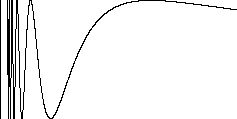
\includegraphics{images/varsavskilok.pdf}
% \caption[caption za v kazalo]{Dolg caption pod sliko}
  \caption[Primer vektorske slike.]{Relacije pokritja v trditvi~\ref{trd:pokritja} lahko prikažemo z grafom.}
  \label{fig:varsavski_lok}
\end{figure}

\begin{figure}[h]
  \centering
  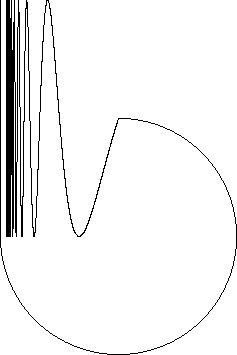
\includegraphics{images/varsavska_kroznica.pdf}
% \caption[caption za v kazalo]{Dolg caption pod sliko}
  \caption[Primer vektorske slike.]{Relacije pokritja v trditvi~\ref{trd:pokritja} lahko prikažemo z grafom.}
  \label{fig:varšavski}
\end{figure}

\begin{definicija}
Množici, ki jo lahko parametriziramo na naslednji način:
\[ p(t) = \begin{cases}
  (t, sin(\frac{1}{t}), & \mbox{ če $t \in (0, 1) $}\\
 (2-t, -(sin(1) +1)t +2sin(1) +2). & \mbox{ če $t \in [1, 2]$}\\
  (0, 3t-8), & \mbox{ če $t \in (2, 3]$.}
  \end{cases}
  \]
\end{definicija}

\begin{trditev}
Varšavska krožnica je prostor Šarkovskega.
\end{trditev}
\begin{proof}
Varšavsko krožnico $X$ lahko parametriziramo z zvezno bijektivno preslikavo $p:I \to X$. Naj bo $f: X \to X$ zvezna funkcija. Ker je funkcija $p$ bijektivna, je funkcija $\widehat{f} = p^{-1} \circ f \circ p : I \to I$ dobro definirana. Trdimo, da je funkcija $\widehat{f}$ zvezna. Ker je funkcija $p$ bijekcija, imata funkciji $f$ in $\widehat{f}$ enake periode. Ker je interval $I$ prostor Šarkovskega, je tudi $X$ prostor Šarkovskega. 

Prepričati se moramo samo še, da je funkcija $\widehat{f}$ res zvezna. Naj bo $t \in I$ poljubna točka intervala $I$ in naj bo $U \in I$ odprta krogla okoli točke $\widehat{f}(t) = (p^{-1} \circ f \circ p)(t)$. Množoco robnih točk krogle $U$ označimo z $A$. Velja $|A| \leq 2$. Ker ima $X$ lastnost $T_2$, so točke zaprte množice in zato je množica $X - p(A)$ odprta podmnožica prostora $X$, ki vsebuje točko $(f \circ p)(t)$. Povezano komponento množice $(f \circ p)^{-1}$, ki vsebuje točko $t$ označimo z $W$. Množica $W$ je odprta podmnožica intervala $I$, saj je funkcija $(f \circ p)$ zvezna. Sedaj obravnavamo množico $\left(p \circ \widehat{f}\right) (W) = (f \circ p)(W) \subset X - p(A)$. Ker je množica $W$ povezava s potmi, je vsebovana v tisti komponenti za povezanost s potmi množice $X-p(A)$, ki vsebuje $(f \circ p)(t)$. 
Prepričali se bomo, da je ta komponenta kar enaka $p(U)$. To je res, saj komponenta vsebuje $p(U)$ in ne more vsebovati nobene druge točke. Denimo, da vsebuje še kakšno drugo točko $x$. Potem vsebuje pot od $x$ do $p(t)$. Ta pot pa  
\end{proof}


%V tem poglavju zapišemo definicijo prostora Šarkovskega. Pokažemo, da je lastnsot prostora Šarkovskega topološka lastnost ( če je X prostor Šarkovskega in je Y homeomorfen prostoru X, je tudi Y prostor Šarkovskskega. Retrakt prostora Šarkovskega je prostor Šarkovskega. Prikažemo nekaj primerov in protiprimerov.

%Ko dokažemo izrek, je naravno, da se vprašamo, ali se da mogoče izrek posplošiti. Lahko se vprašamo, kako se izrek spremeni, če spremenimo predpostavke izreka. Obstaja več posplošitev izreka, ki namesto zveznih funkcij na realnih številih obravnavajo funkcije, ki slikajo nek topološki prostor nazaj vase. V teh primerih lahko periode funkcij ne sledijo nujno Šarkovskemu zaporedju. Kadar pa velja, da za vsako funkcijo $f:X \to X$, ki ima točko periode $m$ obstaja tudi točka periode $l$ za vsak $l \triangleleft m$, imenujemo prostor $X$ prostor Šarkovskega. 
%#############  LINEARNI KONTINUUM JE PROSTOR ŠARKOVSKEGA ##############
%https://en.wikipedia.org/wiki/Order_topology
%https://planetmath.org/aspaceisconnectedundertheorderedtopologyifandonlyifitisalinearcontinuum
%http://mathcenter.spb.ru/nikaan/2019/topology/4.pdf
%http://www.math.buffalo.edu/~badzioch/MTH427/_static/mth427_notes_4.pdf

\section{Linearni kontinuum je prostor Šarkovskega}
V tem poglavju bomo spoznali topologijo urejenih prostorov in posebne urejene prostore s topologijo urejenih prostorov, ki jih imenujemo linearni kontinuum. Gre za neke vrste posplošitev premice realnih števil. Pokazali bomo, da je linearni kontinuum prostor Šarkovskega.

Naj bo množica $X$ urejena s strogo linearno relacijo $<$. Za dana elementa $a, b \in X$, za katera velja neenakost $a<b$, lahko definiramo štiri podmnožice prostora $X$, ki jih imenujemo intervali s krajišči $a$ in $b$. To so:
 Na množici $X$ imamo dve vrsti odprtih množic, ki ju zapišemo na naslednji način:
\begin{equation*} %\label{eq1}
\begin{split}
(a, b) &= \{x \in X: a< x <b\} \\ 
(a, b] &= \{x \in X: a< x \leq b\} \\ 
[a, b) &= \{x \in X: a \leq x< b\} \\ 
[a, b] &= \{x \in X: a \leq x \leq b\}
\end{split}
\end{equation*}

\begin{definicija}
\emph{Linearni kontinuum} je linearno urejena množica $S$, ki ima naslednji lastnosti:
\begin{enumerate}
\item Vsaka navzgor omejena podmnožica $A \subset S$ ima najmanjšo zgornjo mejo v $S$,
\item za vsaki dve števili $x, y \in S$ obstaja število $z \in S$, za katerega je $x<z<y$.
\end{enumerate}
\end{definicija}

\begin{primer}
Enotski kvadrat $[0, 1] \times [0, 1]$ 
\end{primer}

\begin{trditev}
Strogo linearno urejena množica $X$ s topologijo urejenih množic je linearni kontinuum natanko tedaj, ko je povezana.
\end{trditev}
\begin{proof}
Predpostavimo, da je prostor $X$ s topologijo urejenih množic linearni kontinuum. Dokazali bomo, da je prostor $X$ povezan.  
\end{proof}

\begin{izrek}
Naj bo $f : X \to Y$ zvezna funkcija, kjer je $X$ povezan prostor in $Y$ urejen prostor s topologijo urejenih množic. Če sta $a$ in $b$ dve točki v prostoru $X$ in je $r$ točka v prostoru $Y$, ki leži med točkama $f(a)$ in $f(b)$, potem obstaja točke $c \in X$, da velja $f(c) = r$.
\end{izrek}
\begin{proof}
Privzemimo predpostavke izreka. Množici $=f(X) \cap (-\infty, r)$ in $B=f(X) \cap (r, \infty)$ sta disjunktni in neprazni, saj ena množica vsebuje točko $f(a)$, druga pa točko $f(b)$. Obe sta odprti v $f(X)$ saj smo ju dobili kot presek odprtega intervala z množico $f(X)$. Če ne obstaja taka točke $c \in X$, da je $f(c) = r$, potem je $f(X)$ unija množic $A$ in $B$. Na ta način smo dobili separacijo množice $f(X)$, kar pa je protislovje, saj je slika povezane množice z zvezno preslikavo povezana.
\end{proof}

\begin{lema}
Naj bo $L$ linearni kontinuum v topologiji urejenih množic. Naj bosta $I$ in $J$ zaprta intervala v $L$ in $f:L \to L$ zvezna funkcija. Če je $J \subset f(I)$, obstaja zaprt interval $K \subset I$, za katerega je $f(K) = J$.
\end{lema}
\begin{proof}
Izberemo taki točki $p, q \in I$, da velja $p<q$ in $J=[f(p), f(q)]$ ali $J=[f(q), f(p)]$. Definiramo točko $p \leq r < q$:
$$r= \sup\{x \in [p, q] : f(x) = f(p)\}.$$
Trdimo, da je $f(r) = f(p)$. V nasprotnem primeru obstaja odprta množica $V$, ki vsebuje točko $f(r)$ in ne vsebuje točke $f(p)$.To je res, ker je prostor $L$ Hausdorffov. Zaradi zveznosti funkcije $f$ obstaja taka odprta okolica $U$ točke $r$, da je $f(U) \subset V$. Ker je $L$ linearni kontinuum obstaja točka $p \leq r' < r$, da je interval $[r', r]$ vsebovan v množici $U$. Torej je $f([r', r]) \subset V$, kar pomeni, da $f(p) \notin f([r', r])$. To pa je protislovje z definicijo točke $r$ kot supremum množice.
Sedaj definiramo $r<s \leq q$:
$$r= \inf\{x \in [r, q] : f(x) = f(q)\}.$$ 
Enako kot prej se prepričamo, da je $f(s) = f(q)$. Zapišimo $Q = [r, s]$ in pokažimo, da je $f(Q) = J$. Izrek o vmesni vrednosti zagotavlja, da je interval $J$ vsebovan v množici $f([r, s])$. Velja tudi $f([r, s]) \subset J$, saj v nasprotnem primeru obstaja $r<x<s$, za katerega velja $f(x) \notin J$. Če je $f(x) < f(p) < f(q)$ ali $f(q) < f(p) < f(x)$, potem po izreku o vmesni vrednosti obstaja tak $x'$, da velja $r<x<x'<s$ in $f(p) = f(x')$. to pa je protislovje z definicijo točke $r$ kot supremum. Če je $f(x) < f(q) < f(p)$ ali $f(p) < f(q) < f(x)$, to privede do protislovja z definicijo točke $s$ kot infimum. To pomeni, da res felja $J = f(Q)$.
\end{proof}

\begin{lema}
Naj bo $L$ linearni kontinuum v topologiji urejenih množic. Naj bosta $I$ zaprt interval v $L$ in $f:L \to L$ zvezna funkcija. Če je $I \subset f(I)$, potem ima $f$ negibno točko $x \in I$.
\end{lema}
\begin{proof}
S pomočjo leme~\ref{} ugotovimo, da obstaja zaprt interval $Q \subset I$, za katerega je $f(Q) = I$. Pokazali bomo, da ima funkcija $f$ negibno točko v intervalu $Q$. Predpostavimo, da funkcija $f$ na intervalu $Q$ nima negibne točke. Potem lahko zapišemo $Q = A \cup B$, kjer je:
\begin{equation*} %\label{eq1}
\begin{split}
A &= \{x \in L : x < f(x)\}, \\ 
B &= \{x \in L : x > f(x)\}.
\end{split}
\end{equation*}
Trdimo, da je množica $A$ odprta. Za vsako točko $x \in A$ lahko izberemo točko $z \in (x, f(x))$ in odprto okolico $U \subset  (-\infty, z)$ točke $x$, za katero velja $f(U) \subset (z, \infty)$. Ker je množica $U$ podmnožica množoce $A$, je točka $x$ notranja točka množice $A$. Množica $A$ je odprta. Podobno lahko dokažemo, da je množica $B$ odprta. Množici $Q \cap A$ in $Q \cap B$ sta odprti podmnožici množice $Q$ za kateri velja $Q = (Q \cap A) \cup (Q \cap B)$. Radi bi videli, da sta množici $Q \cap A$ in $Q \cap B$ neprazni. Zapišimo $I = [c, d]$. Ker je $f(Q) = I$, obstaja $x' \in Q$, za katerega je $f(x') =d$. Ker $f$ nima fiksne točke na $Q$, je $x' \neq d$. Interval $Q$ je pomnožica intervala $I$, zato velja $x' < f(x') = d$, kar pomeni, da je $x' \in Q \cap A$. Analogno poiščemo točko $x'' \in Q - \{c\}$ z lastnostjo: $f(x'') = c$ in $x'' \in Q \cap B$. Torej, množici $Q \cap A$ in $Q \cap B$ tvorita separacijo povezanega prostora $Q$, kar je protislovje. Funkcija $f$ ima negibno točko v intervalu $Q$.
\end{proof}



% Literatura:
% Primer navajanja na http://www.fmf.uni-lj.si/storage/24240/LiteraturaM.pdf,
% ampak bi moral stil poskrbeti za vse. Reference se uredijo po abecedi.
% Če nobena izbira izmed @book, @atricle,... ni ok, potem se lahko vse napiše v
% @misc pod note={} in deluje tako kot normalen LaTeX.
% Komentar v bib datoteki se naredi samo s parom { }
% Za urejanje literature avtor priporoča program Jabref, ki zna tudi avtomatsko
% okrajšati imena revij. Za pravilno sortiranje vnosov brez avtorja, uporabite
% polje key={ }, kot v primeru.
% V primeru napak ustvarite issue na GitHubu ali pišite na jure.slak@fmf.uni-lj.si.
\cleardoublepage                           % na desni strani
\phantomsection                            % da prav delujejo hiperlinki
\addcontentsline{toc}{section}{\bibname}   % dodajmo v kazalo
\bibliographystyle{fmf-sl}                 % uporabljen stil je v datoteki fmf-sl.bst, na voljo tudi angleška verzija
%\bibliography{\literatura}                 % literatura je v datoteki, definirani na začetku
% TeXStudio zmede \ zgoraj, tako da lahko notri napišeš dejansko ime .bib datoteke, če ti
% ne delajo predlogi citatov.

% Za stvarno kazalo
\cleardoublepage                           % na desni strani
\phantomsection                            % da prav delujejo hiperlinki
\addcontentsline{toc}{section}{\indexname} % dodajmo v kazalo
\printindex

\end{document}


